% Progetto di ingegneria del software - Relazione (pdf)

\documentclass[twoside,openright,titlepage,fleqn,headinclude,12pt,a4paper,BCOR=5mm,footinclude]{scrbook}

\usepackage{float}
\usepackage{placeins}
\usepackage{array}
\usepackage[nottoc]{tocbibind}
\usepackage[utf8]{inputenc} 
\usepackage[T1]{fontenc} 
\usepackage[english]{babel}
\usepackage{csquotes}
\usepackage[fleqn]{amsmath}  
\usepackage{ellipsis}
\usepackage{listings}
\usepackage{subfig}
\usepackage{caption}
\usepackage{appendix}
\usepackage{siunitx}
\usepackage[pdftex]{graphicx}
\usepackage[eulerchapternumbers,linedheaders,subfig,beramono,eulermath,parts,dottedtoc]{classicthesis}
\usepackage{geometry}

\newlength{\abcd} 
\setlength{\extrarowheight}{3pt} 
\captionsetup{format=hang,font=small}

\geometry{
	a4paper,
	ignoremp,
	bindingoffset = 1cm, 
	textwidth     = 13.5cm,
	textheight    = 21.5cm,
	lmargin       = 3.5cm, 
	tmargin       = 4cm    
}

\lstset{
  	frame=tb,
	language=Matlab,
  	aboveskip=3mm,
  	belowskip=3mm,
  	showstringspaces=false,
  	columns=flexible,
  	basicstyle={\small\ttfamily},
  	numbers=none,
  	breaklines=true,
  	breakatwhitespace=true,
  	tabsize=3
}

\begin{document}
\frenchspacing
\raggedbottom
\pagenumbering{roman}
\pagestyle{plain}

\begin{titlepage}
    \begin{center}
        \large
        \hfill        
        \vfill
        \begingroup
            \includegraphics[scale=0.15]{images/logo}\\
            Scuola di Ingegneria\xspace\\
            Corso di Laurea in Ingegneria Informatica\xspace\\
            \vspace{0.5cm}
            \vspace{0.5cm}
            \textbf{Progetto di Ingegneria del Software}\\
            \vspace{0.5cm}
        \endgroup
        \vfill
        \begingroup
        Applicazione per la gestione di campionati Fanta-sports \xspace \\ $\ $\\
	\bigskip
	\bigskip
      \endgroup
      \spacedlowsmallcaps{Rialti Jacopo, Tescaro Rocco \xspace}
      \vfill 
      \vfill
	\bigskip
	\bigskip
      \vfill
      \vfill
      \vfill
      \vfill
      \vfill
      \vfill
      \vfill
      \vfill
      Anno Accademico 2023-2024
	\end{center}        
\end{titlepage}   

\newpage
\thispagestyle{empty}
\hfill
\vfill
\noindent Rialti Jacopo, Tescaro Rocco \xspace: 
\textit{Applicazione per la gestione di campionati Fanta-sports \xspace,} 
Ingegneria del Software \xspace, \textcopyright\ Anno Accademico 2023-2024 \xspace

\pagestyle{scrheadings}
\cleardoublepage
\clearpage
\pagenumbering{arabic}
\tableofcontents
\cleardoublepage

\clearpage
\chapter{Introduzione}
\section{Obiettivi del progetto}
Il progetto corrente nasce con l'obiettivo di realizzare un'applicazione per la gestione di campionati Fanta-sports, in particolare di calcio.
E' ormai diffusissimo il fenomeno dei campionati fanta-sports, dove i giocatori hanno la possibilità di amministrare le proprie squadre favorite e 
sfidarsi con altri giocatori. L'applicazione nasce appunto con l'obiettivo di fornire un servizio/strumento per l'organizzazione di campionati privati e
per estensione anche pubblici.

L'applicazione permette di creare leghe private di fanta-soccer, ovvero un campionato in cui gli utenti ad invito possono creare una squadra virtuale, 
composta da giocatori reali, e sfidarsi, con anche la possibilità di estendere le regole del campionato personalizzandole o possibilmente collegare
un proprio database all'applicazione rendendo possibile la creazione di campionati di altri sport.

Le principali funzionalità dell'applicazione sono: la possibilità di creare un campionato, di invitare altri utenti a partecipare, di avviare un'asta 
e comporre una squadra, di definire modalità di punteggio e regole del campionato, di visualizzare la classifica e i risultati delle partite.

\section{Elementi del progetto}
Il progetto è composto da:
\begin{itemize}

    \item \textbf{Utente giocatore (User)}: è l'utente che partecipa al campionato, partecipare all'asta, comporre e gestire la propria squadra, 
    visualizzare la classifica e i risultati delle partite. Non può modificare creare un campionato o modificare le regole di uno esistente 
    (nemmeno se partecipante dello stesso).
    
    \item \textbf{Utente amministratore (Creator)}: è l'utente che crea un campionato, invita altri utenti a partecipare, avvia l'asta, modifica le regole. 
    Scelte le regole, l'utente amministratore non può più modificarle a campionato iniziato. Ha anche il compito di fornire il database dei giocatori 
    (reali) e il database delle valutazioni per il calcolo del punteggio.
    
    \item \textbf{Squadra (Team)}: Rappresenta la squadra di un utente in un determinato campionato. Ogni squadra è composta da un insieme di giocatori reali selezionati dall'utente durante l'asta. Ogni squadra ha un proprietario (l'utente che l'ha creata) e appartiene a una lega specifica. Le squadre accumulano punti in base alle prestazioni dei loro giocatori nelle formazioni nelle partite reali, secondo le regole a punti. Ogni squadra ha anche una formazione, che è l'insieme di giocatori selezionati per giocare in una determinata giornata del campionato. La formazione può essere modificata dall'utente proprietario prima dell'inizio di ogni giornata.
     
     \item \textbf{Giocatore sportivo (Player)}: Rappresenta un giocatore reale nel contesto del campionato. Ogni giocatore ha un punteggio che determina le sue prestazioni nelle partite reali. Queste prestazioni influenzano i punti accumulati dalle squadre nelle quali il giocatore è stato selezionato. Ogni giocatore può appartenere a più squadre e leghe, a seconda delle scelte degli utenti durante l'asta. Inoltre, un giocatore può essere parte della formazione di una squadra, che è l'insieme di giocatori selezionati per giocare in una determinata giornata del campionato.

     \item \textbf{Lega (League)}: Rappresenta un campionato nel contesto del gioco. Ogni lega è creata da un utente amministratore e può avere un numero specifico di partecipanti. Le leghe hanno regole specifiche, come il numero di giocatori in una formazione e il numero di utenti giocatori partecipanti. Ogni lega ha anche una data di inizio e che indica quando sarà la prossima giornata. Inoltre, ogni lega ha un insieme completo di giocatori reali che possono essere selezionati dagli utenti durante l'asta. Infine, ogni lega ha un insieme di squadre, ciascuna delle quali appartiene a un utente specifico che partecipa alla lega.
     
\end{itemize}

\section{Estendibilità del progetto}
Il progetto è stato pensato per essere estendibile, in particolare per quanto riguarda la possibilità di creare campionati di altri sport.
Per fare ciò è necessario fornire un database di giocatori e un database di valutazioni per il calcolo del punteggio.

Un'altra possibilità di estensione è la possibilità di avviare leghe pubbliche, ovvero leghe il cui accesso è disponibile a tutti gli utenti 
dell'applicazione, senza quindi necessità di invito da parte dell'amministratore. A questa estensione è legata anche la possibilità di visualizzare una
classifica globale, ovvero una classifica che tiene conto di tutti i campionati pubblici attivi.

In ultima istanza è possibile estendere l'applicazione affinchè siano gestite altre regole o tipologie di campionati, idealmente non vincolare dalla regola
dell'immutabilità delle regole a campionato iniziato. 

\chapter{Analisi dei requisiti}
\section{Use Case Diagram}
Il software presenta 2 diversi tipi di attori: lo User e il Creator. Lo user può partecipare ad una lega creata da un altro Creator, gestendo il suo team all'interno della lega. Lo user per diventare un Creator, deve creare un nuova lega, nella quale avrà poi la possibilità di gestire e modificare tutte le varie opzioni, squadre e giocatori all'interno di essa. Lo schema dei casi d'uso sottostante è stato realizzato mediante StarUML secondo lo standard UML.

\begin{figure}[H]
  \centering
  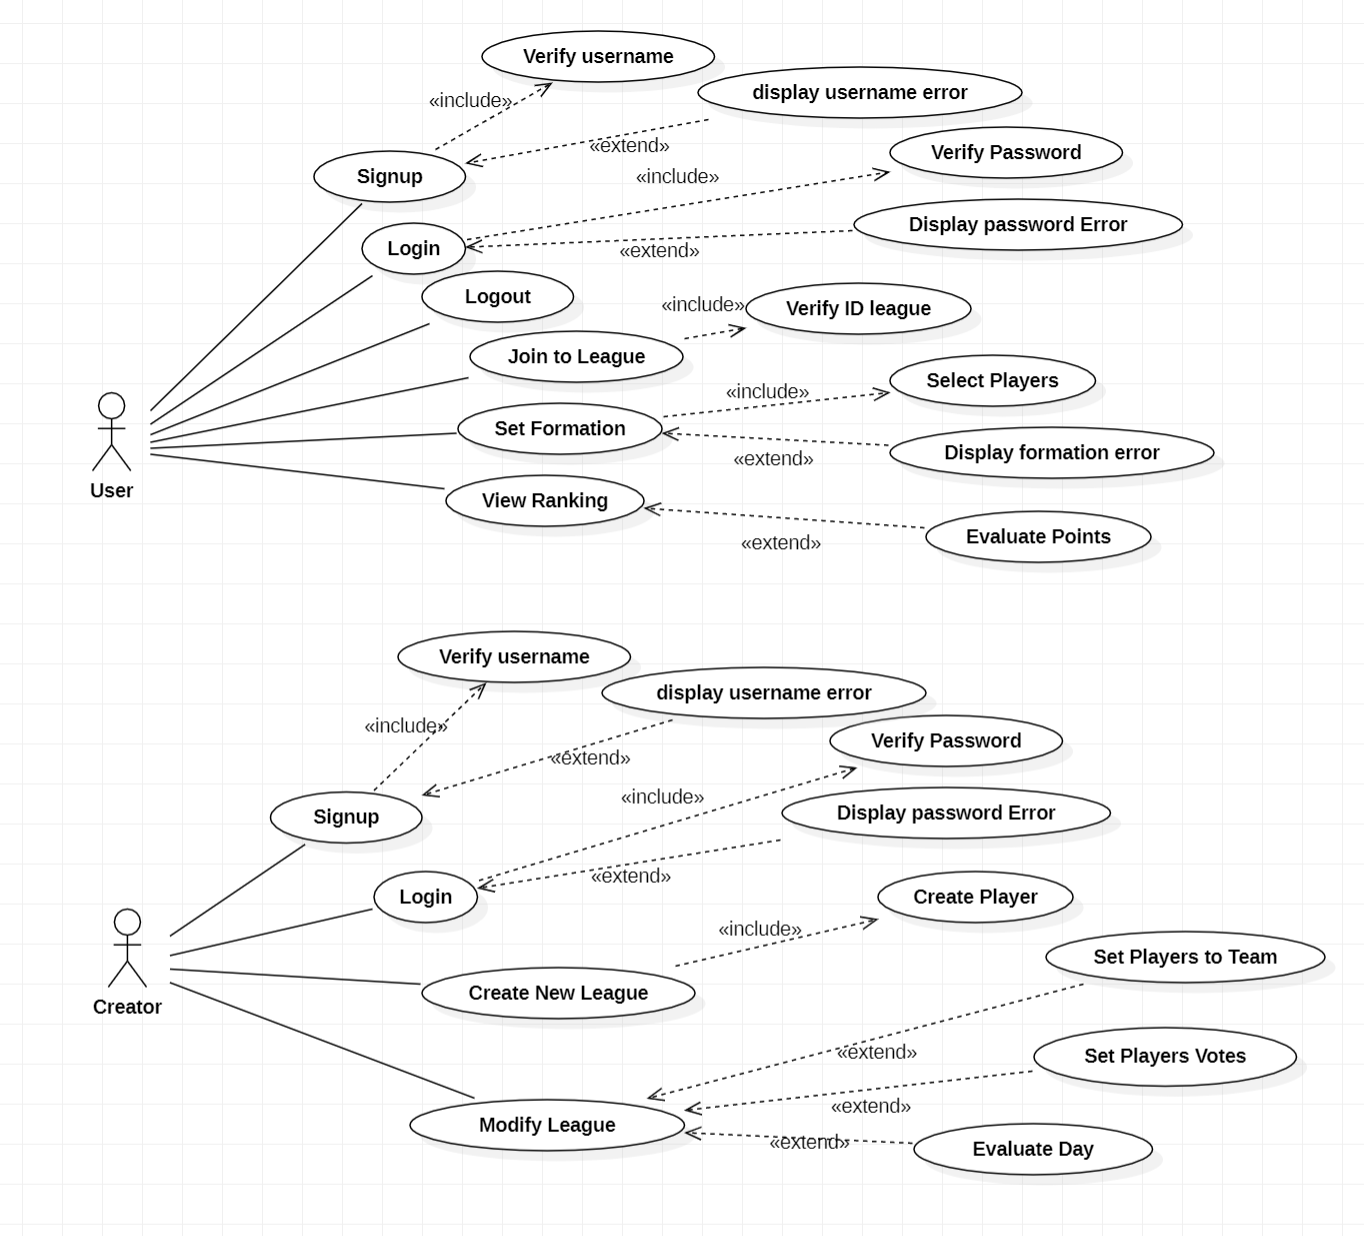
\includegraphics[width=0.8\linewidth]{images/useCaseDia.png}
  \caption{Use Case Diagram}
  \label{fig:Use Case Diagram}
\end{figure}


\section{Use Case Templates}


\subsection{Casi d’uso principali di uno User}

\begin{table}[H]
    \centering
    \begin{tabular}{|>{\raggedright\arraybackslash}m{2.5cm}|>{\raggedright\arraybackslash}m{10cm}|}
        \hline
        \textbf{UC-1} & \textbf{Join to League} \\
        \hline
        \textbf{Descrizione} & Lo user effettua l'accesso alla lega, inserendo l'ID di quest'ultima nell'apposito campo e diventando un partecipante. \\
        \hline
        \textbf{Livello} & User goal \\
        \hline
        \textbf{Attore principale} & User \\
        \hline
        \textbf{Azioni} & 
        1. Lo user, dalla schermata home, inserisce l'ID della lega nel apposito form "Join to League". \newline
        2. Se l'ID è corretto e la capienza della lega non è piena, effettuerà l'accesso. \newline
        3. L'utente è diventato un partecipante della lega e potrà vedere tutte le informazioni di quest'ultima. \\
        \hline
        \textbf{Casi straordinari} & 2a. Nel caso l'ID della lega non corrisponde ad una lega esistente oppure la lega ha già raggiunto il numero dei partecipanti, lo User non potrà partecipare. \\
        \hline
    \end{tabular}
    \caption{Partecipazione dello User ad una lega già creata}
    \label{tab:join_to_league}
\end{table}

\begin{table}[H]
    \centering
    \begin{tabular}{|>{\raggedright\arraybackslash}m{2.5cm}|>{\raggedright\arraybackslash}m{10cm}|}
        \hline
        \textbf{UC-2} & \textbf{Set Formation} \\
        \hline
        \textbf{Descrizione} & Lo user dalla pagina della lega, potrà selezionare i giocatori presenti nel suo team, inserendoli nella rosa per la prossima giornata. \\
        \hline
        \textbf{Livello} & User goal \\
        \hline
        \textbf{Attore principale} & User \\
        \hline
        \textbf{Azioni} & 
        1. Lo user clicca sulla relativa lega dalla schermata home. \newline
        2. Lo user seleziona i giocatori che vuole inserire nella rosa, attraverso un multiple choice. \newline
        3. Lo user, una volta selezionati, clicca su Set Formation, salvando così i giocatori selezionati nella rosa. \\
        \hline
        \textbf{Casi straordinari} & 
        2a. Nel caso in cui il numero di giocatori selezionati non corrisponde al numero di giocatori che devono essere inseriti nella rosa, non potrà cliccare sul pulsante per salvare quest'ultima. \newline
        2b. Se lo user si scorda di inserire la rosa per una determinata giornata, il calcolo della giornata verrà effettuato sull'ultima rosa salvata. \\
        \hline
    \end{tabular}
    \caption{Inserimento della formazione titolare}
    \label{tab:set_formation}
\end{table}

\subsection{Casi d’uso principali di un Creator}

\begin{table}[H]
    \centering
    \begin{tabular}{|>{\raggedright\arraybackslash}m{2.5cm}|>{\raggedright\arraybackslash}m{10cm}|}
        \hline
        \textbf{UC-3} & \textbf{Create New League} \\
        \hline
        \textbf{Descrizione} & Uno user, cliccando sul pulsante nella home page "Create New League", può creare una nuova lega, inserendo tutte le informazioni relative a questo campionato. Lo user dopodiché diventerà Creator di quest'ultima. \\
        \hline
        \textbf{Livello} & User goal \\
        \hline
        \textbf{Attore principale} & Creator \\
        \hline
        \textbf{Azioni} & 
        1. Il creator dalla schermata home clicca su "Create League". \newline
        2. Inserisce le informazioni richieste (nome, numero di partecipanti, pool dei players, start date, etc.). \newline
        3. Clicca su "Create" per creare la lega. \\
        \hline
        \textbf{Casi straordinari} & 2a. Nel caso in cui il Creator imposta dei dati non validi riguardanti il set-up della Lega e clicca su Save, verrà reindirizzato nuovamente sulla stessa pagina ma con tutti i campi azzerati. \\
        \hline
    \end{tabular}
    \caption{Creazione di una nuova lega}
    \label{tab:create_new_league}
\end{table}


\begin{table}[H]
    \centering
    \begin{tabular}{|>{\raggedright\arraybackslash}m{2.5cm}|>{\raggedright\arraybackslash}m{10cm}|}
        \hline
        \textbf{UC-4} & \textbf{Modify League} \\
        \hline
        \textbf{Descrizione} & Il creator può modificare una lega esistente, calcolare il punteggio della giornata, inserire la data della prossima giornata, assegnare giocatori ai vari partecipanti e rimuovere partecipanti. \\
        \hline
        \textbf{Livello} & User goal \\
        \hline
        \textbf{Attore principale} & Creator \\
        \hline
        \textbf{Azioni} & 
        1. Il creator seleziona la lega da modificare dalla schermata home. \newline
        2. Inserisce la data della prossima giornata. \newline
        3. Calcola il punteggio della giornata. \newline
        4. Assegna giocatori ai vari partecipanti. \newline
        5. Rimuove partecipanti, se necessario. \\
        \hline
        \textbf{Casi straordinari} & 
        2a. Nel caso in cui il creator inserisca una data non valida, viene mostrato un messaggio di errore. \newline
        4a. Se l'assegnazione dei giocatori non è valida, viene mostrato un messaggio di errore e il creator deve correggere l'assegnazione. \\
        \hline
    \end{tabular}
    \caption{Modifica di una lega}
    \label{tab:modify_league}
\end{table}

\section{Mockups}
Ecco alcuni Mockups che sono veri e propri screenshot della GUI realizzata a questo proposito.

\subsection{Create league}
\begin{figure}[H]
  \centering
  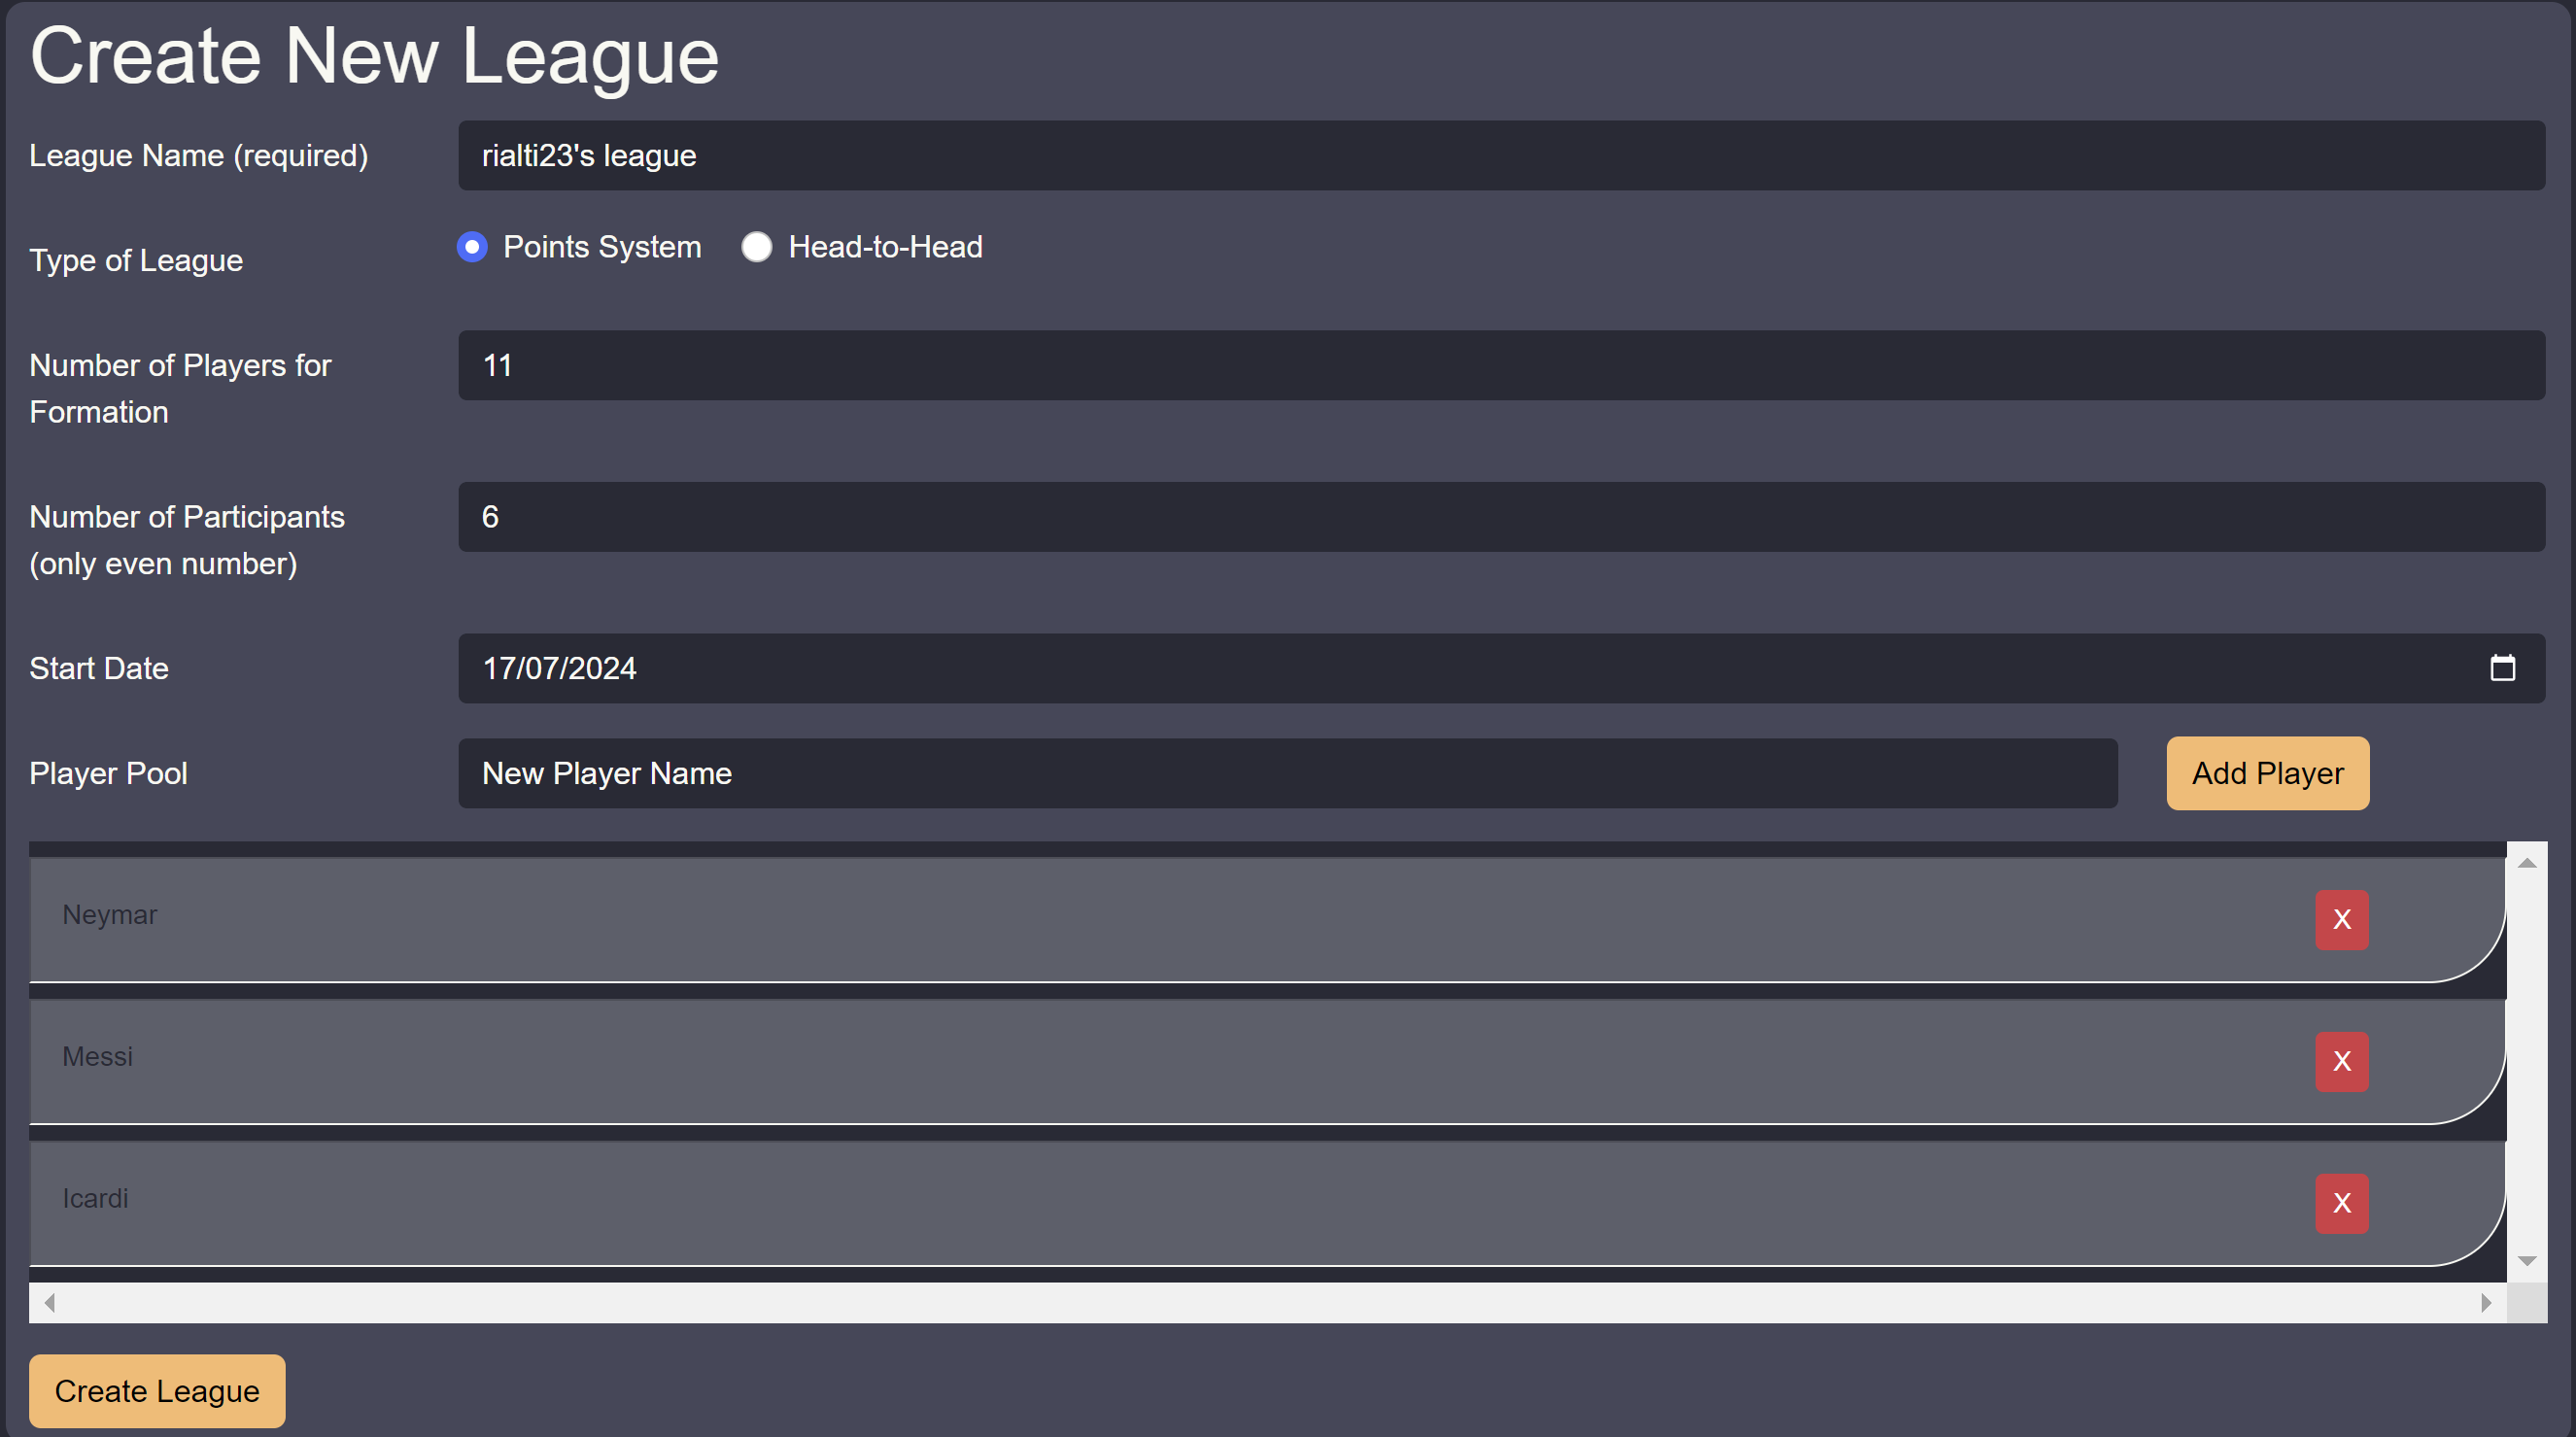
\includegraphics[width=\linewidth]{images/createLeague.png}
  \caption{Crea una nuova lega}
  \label{fig:create}
\end{figure}


\subsection{Join league}
\begin{figure}[H]
  \centering
  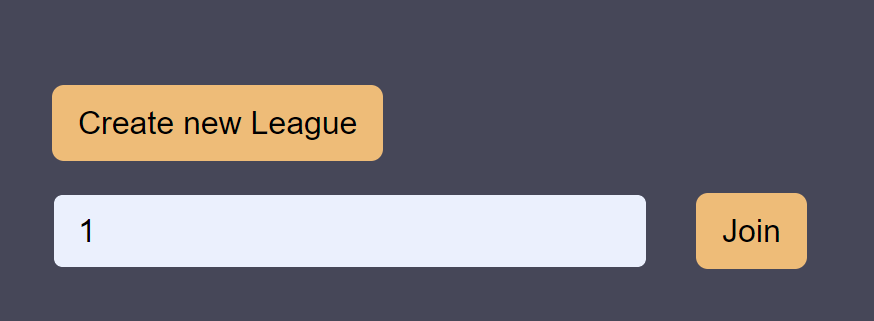
\includegraphics[width=\linewidth]{images/joinLeague.png}
  \caption{Partecipa ad una lega già creata}
  \label{fig:join}
\end{figure}

\subsection{Add Players to a team}

\begin{figure}[H]
  \centering
  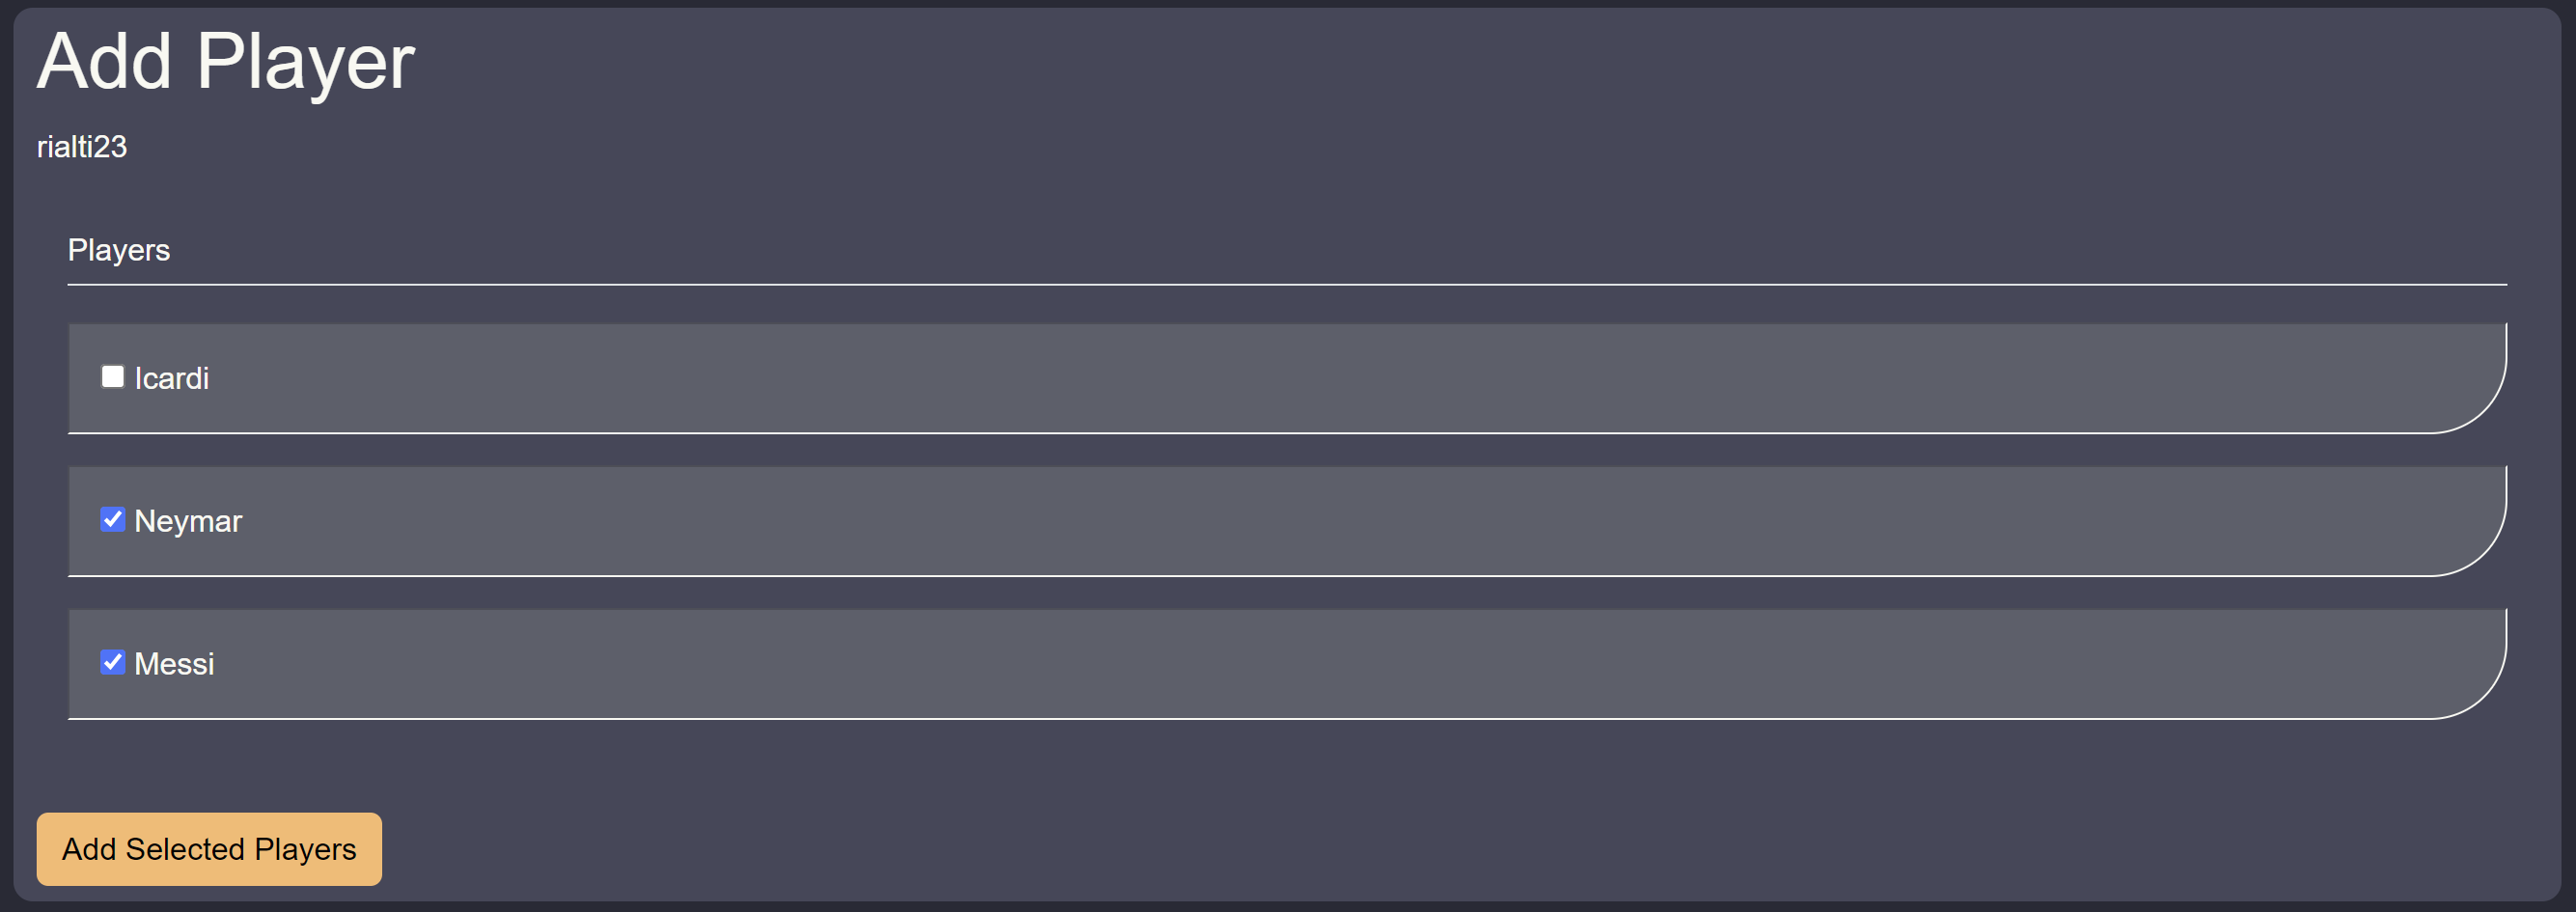
\includegraphics[width=\linewidth]{images/addPlayer.png}
  \caption{Aggiungi giocatori ad un Team}
  \label{fig:addPlayer}
\end{figure}

\subsection{Set Players votes}

\begin{figure}[H]
  \centering
  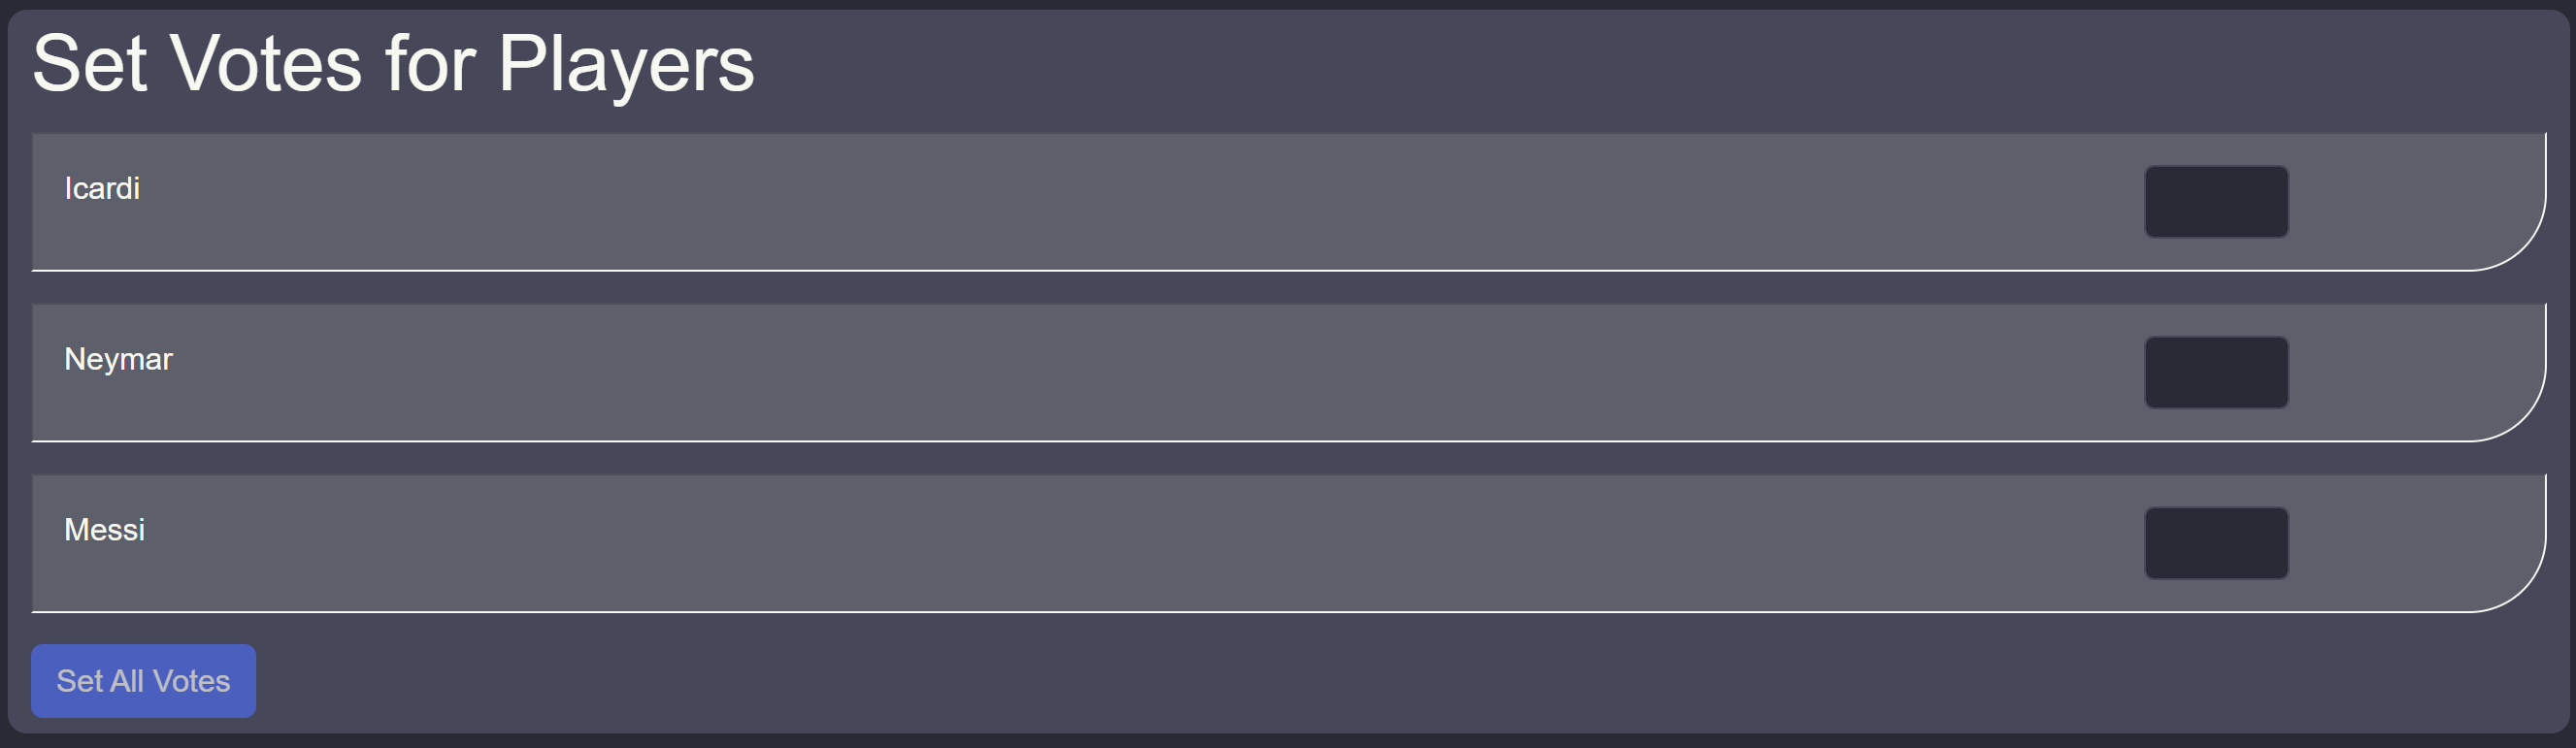
\includegraphics[width=\linewidth]{images/setVotes.png}
  \caption{Assegna le valutazioni a tutti i giocatori della lega}
  \label{fig:setVotes}
\end{figure}

\subsection{Evaluate current Day}

\begin{figure}[H]
  \centering
  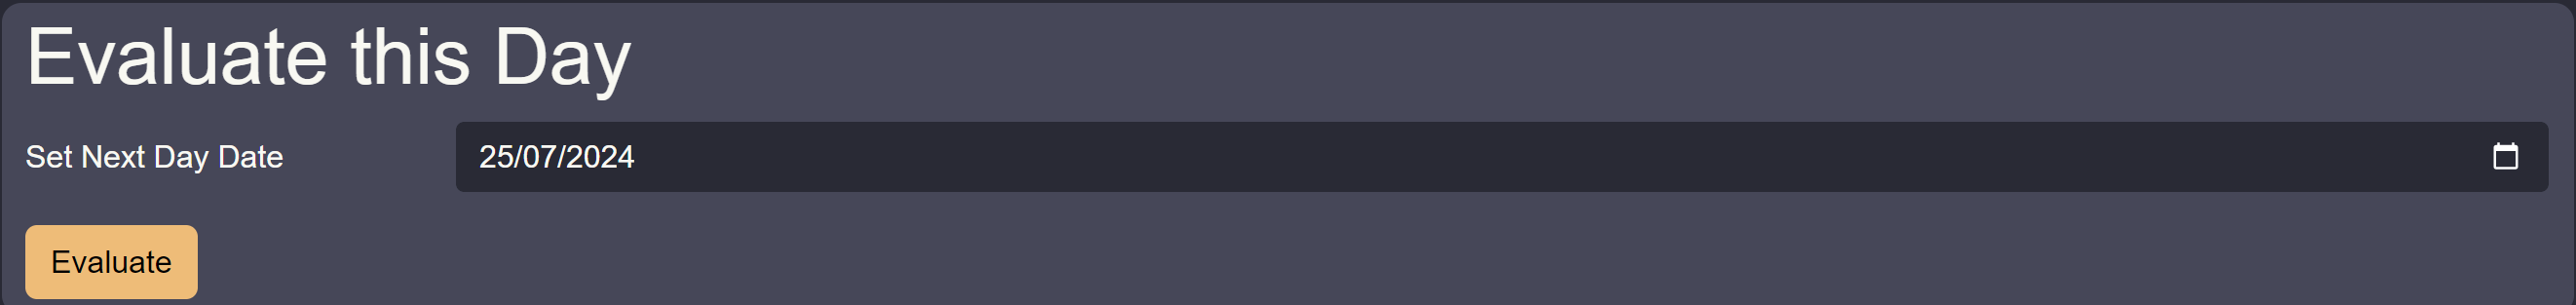
\includegraphics[width=\linewidth]{images/evaluateDay.png}
  \caption{Calcola punteggio giornata e assegna nuova data della prossima}
  \label{fig:evaluate}
\end{figure}

\subsection{Set team Formation}

\begin{figure}[H]
  \centering
  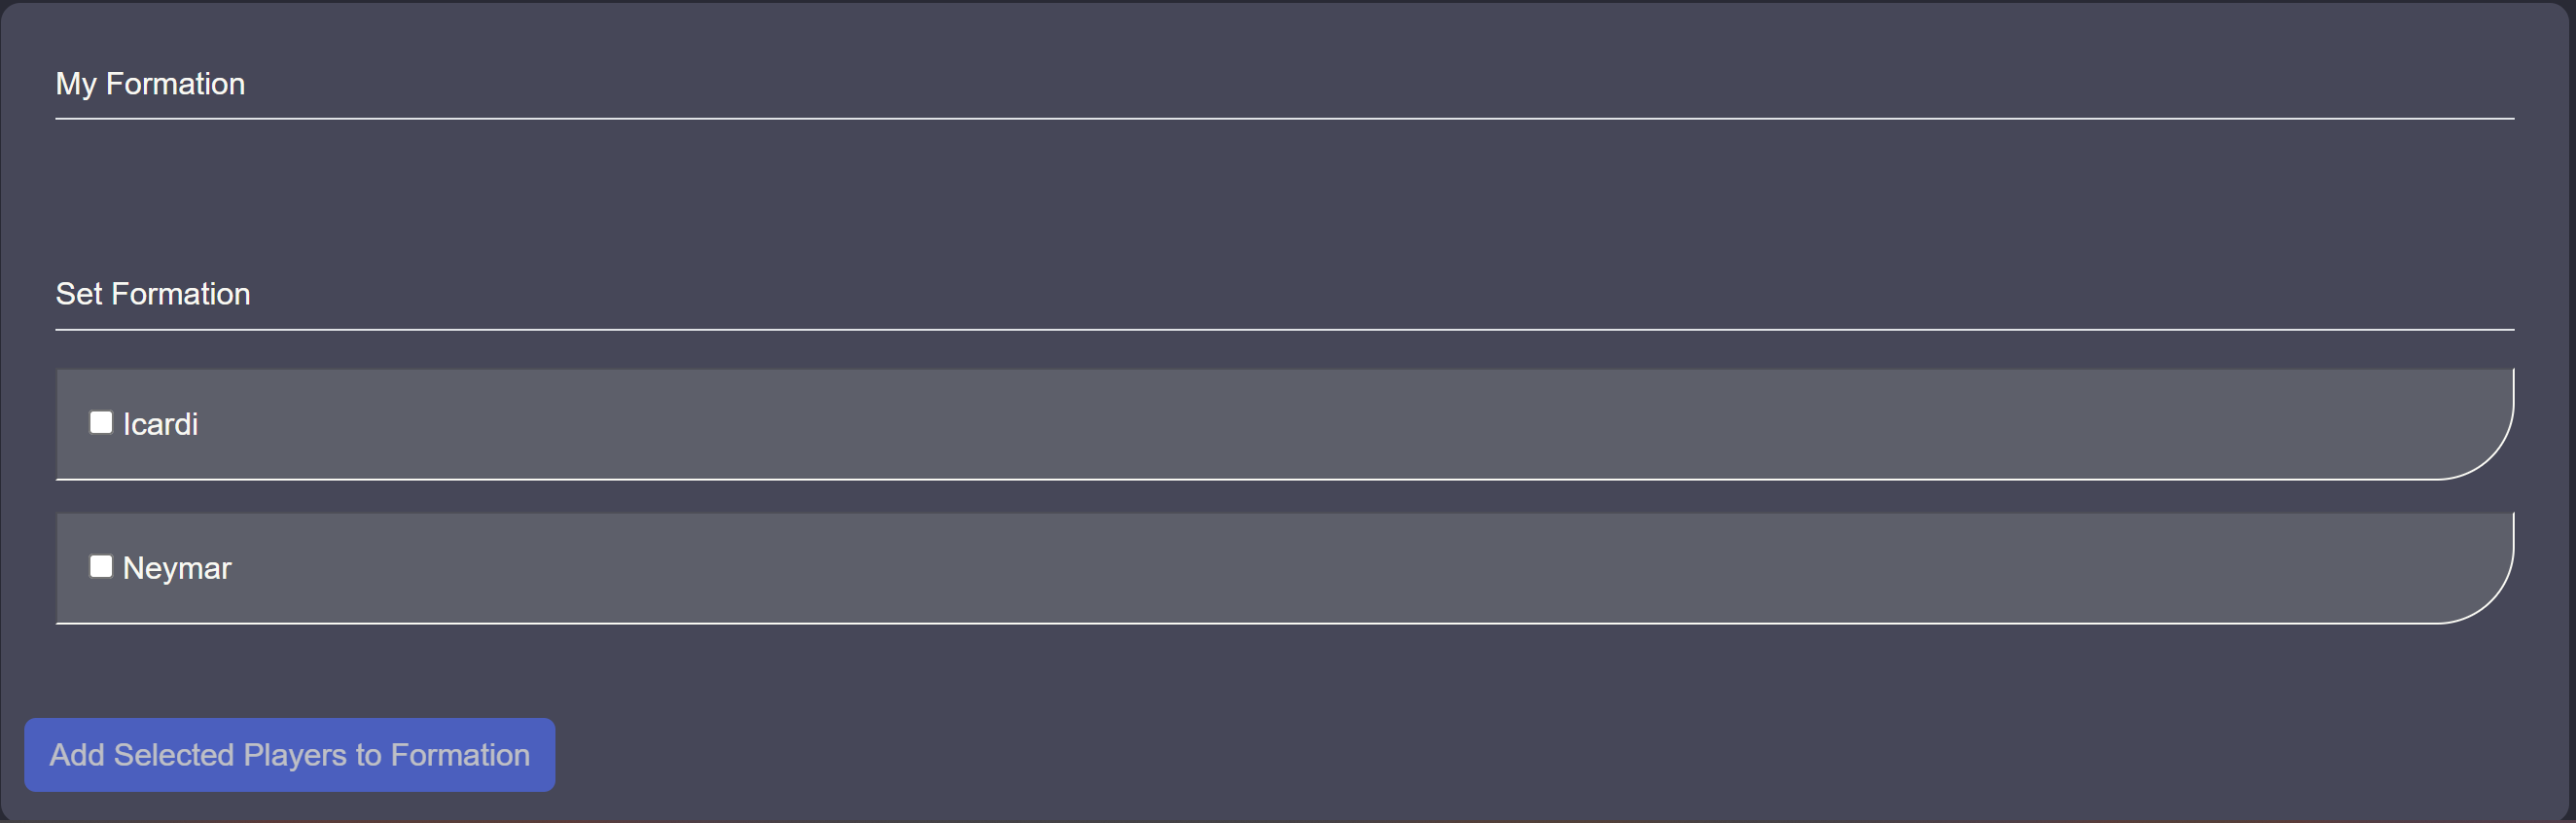
\includegraphics[width=\linewidth]{images/setFormation.png}
  \caption{Seleziona i giocatori da inserire nella formazione titolare}
  \label{fig:setFormation}
\end{figure}

\subsection{League details}

\begin{figure}[H]
  \centering
  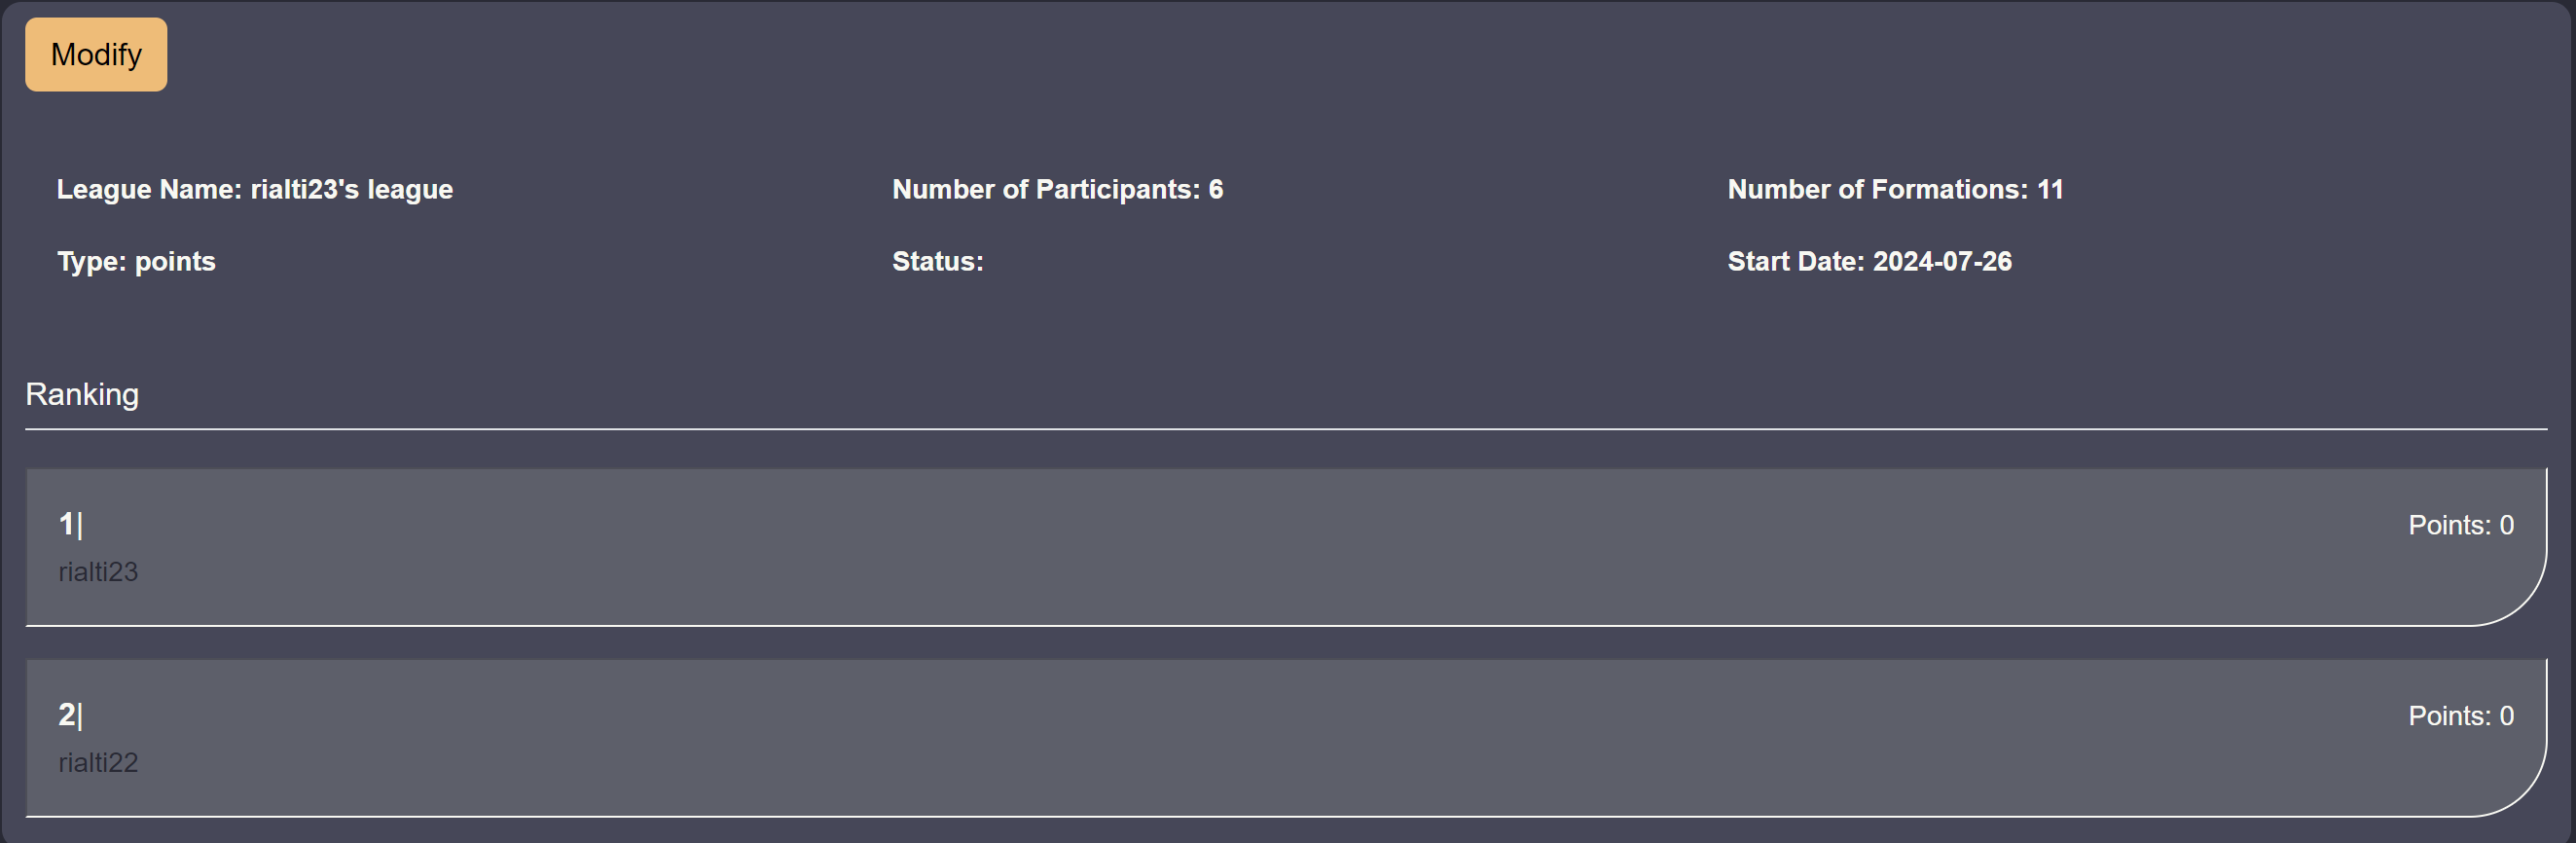
\includegraphics[width=\linewidth]{images/detailLeague.png}
  \caption{Visualizza informazioni riguardo la lega}
  \label{fig:detail}
\end{figure}

\section{Class Diagram}


\begin{figure}[H]
  \centering
  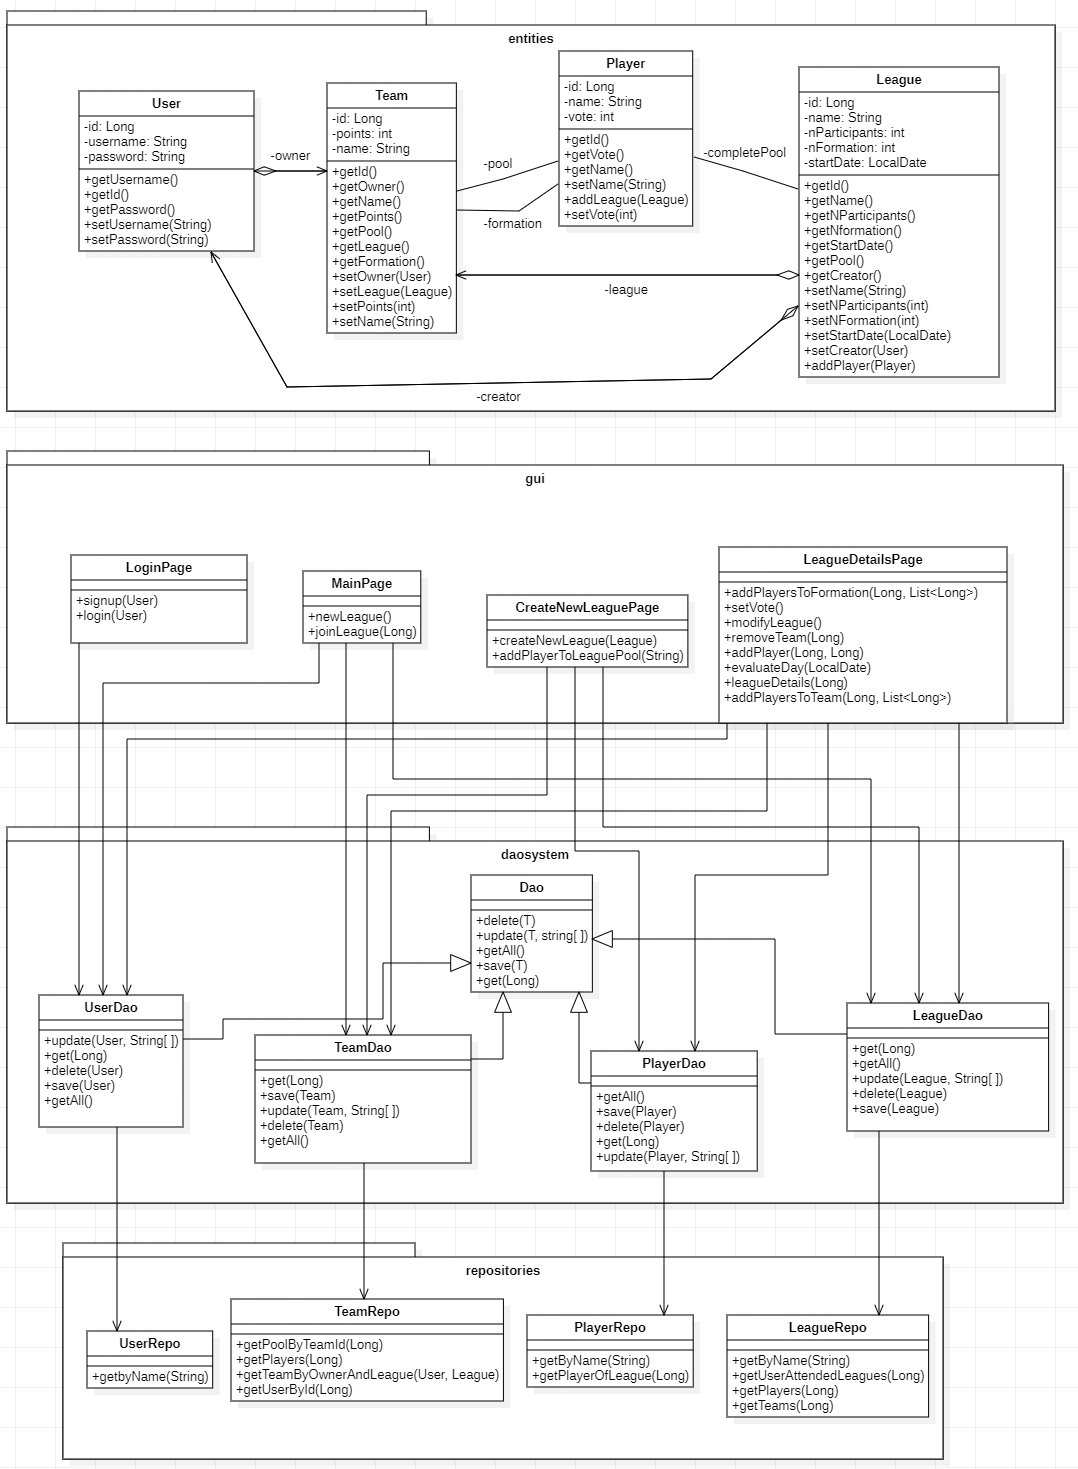
\includegraphics[width=\linewidth]{images/classDia.png}
  \caption{Class Diagram}
  \label{fig:Class Diagram}
\end{figure}



Il codice contiene all'interno tali packages:
\begin{itemize}
    \item entities: rappresenta le varie entità all'interno del software. Contine tutte le classi tramite le quali vengono rappresentati tutti gli oggetti nel software. All'interno delle classi sono definiti gli attributi delle varie entità.
    \item gui: . Contiene le classi che si occupano di modificare i dati, comunicando esclusivamente con dei servizi per poter accedere al database senza farl direttamente. In questo package sono presenti, dunque, tutti i controller per i modelli mappati nel Database.
 
    \item dao:

    \item repositories:

\end{itemize}

\section{DAO Pattern}
Abbiamo utilizzato il Design Pattern DAO in modo che il client non possa intergire direttamente con il Database.


\begin{figure}[H]
  \centering
  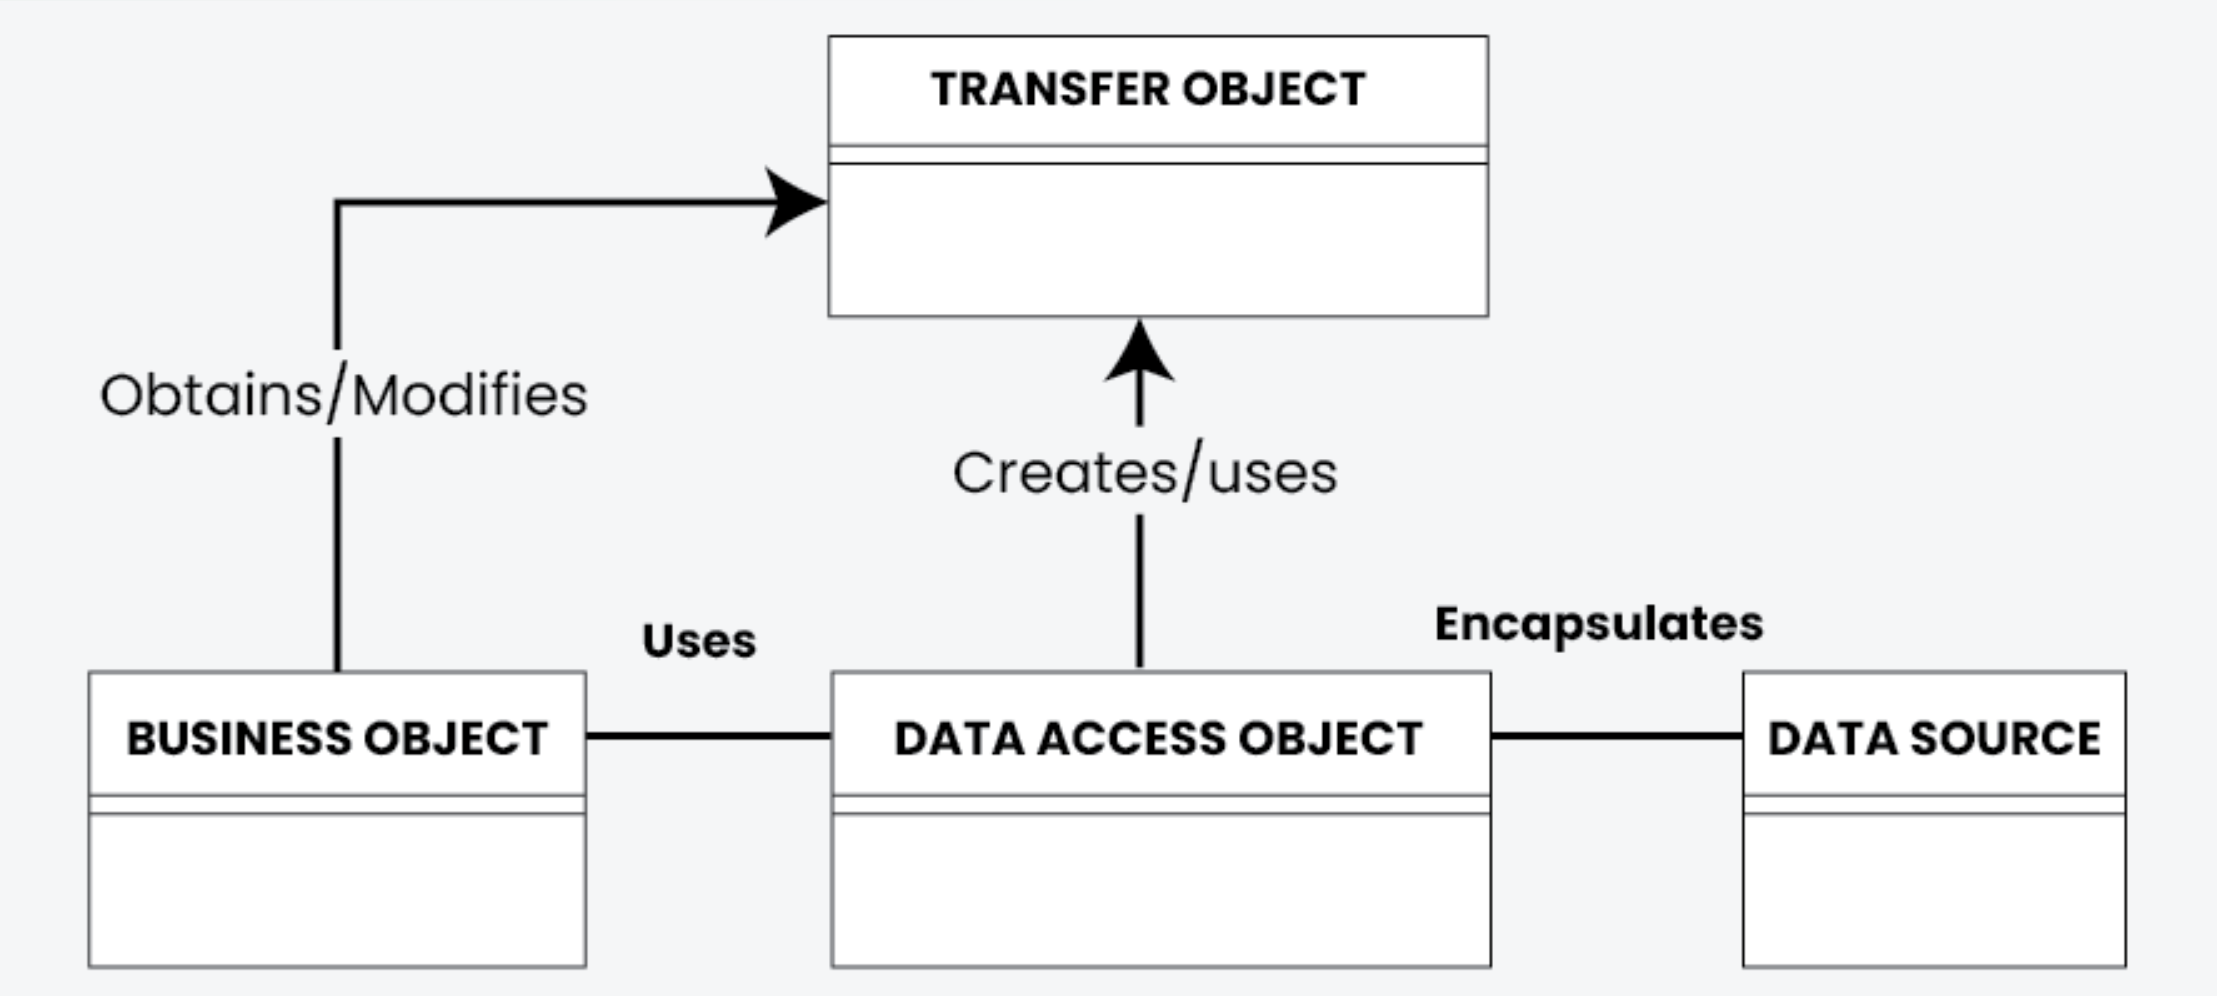
\includegraphics[width=\linewidth]{images/daoDiagram.png}
  \caption{General DAO Diagram}
  \label{fig:Dao Diagram}
\end{figure}



Il pattern architetturale DAO (Data Access Object) viene utilizzato per gestire la persistenza dei dati registrati in un database. La persistenza si riferisce alla capacità di un dato di "sopravvivere" all'esecuzione di un programma, ovvero di continuare a esistere e rimanere coerente anche dopo la fine del programma stesso. Questo pattern ha lo scopo di separare la logica di accesso ai dati dal resto dell'applicazione. È progettato per isolare il codice che si occupa dell'accesso e della manipolazione dei dati da quello che implementa la logica di business del nostro software. La classe DAO definisce e offre metodi CRUD (Create, Read, Update, Delete) per i dati presenti nel database.

Le classi che sfruttano il DAO e che sono presenti nel DB sono le seguenti:

\begin{itemize}
    \item User;
    \item Team;
    \item League;
    \item Player.
    
\end{itemize}

\section{Entity Relationship Diagram}
Questo è il diagramma ER del progetto, con le varie cardinalità delle relazioni.

\begin{figure}[H]
  \centering
  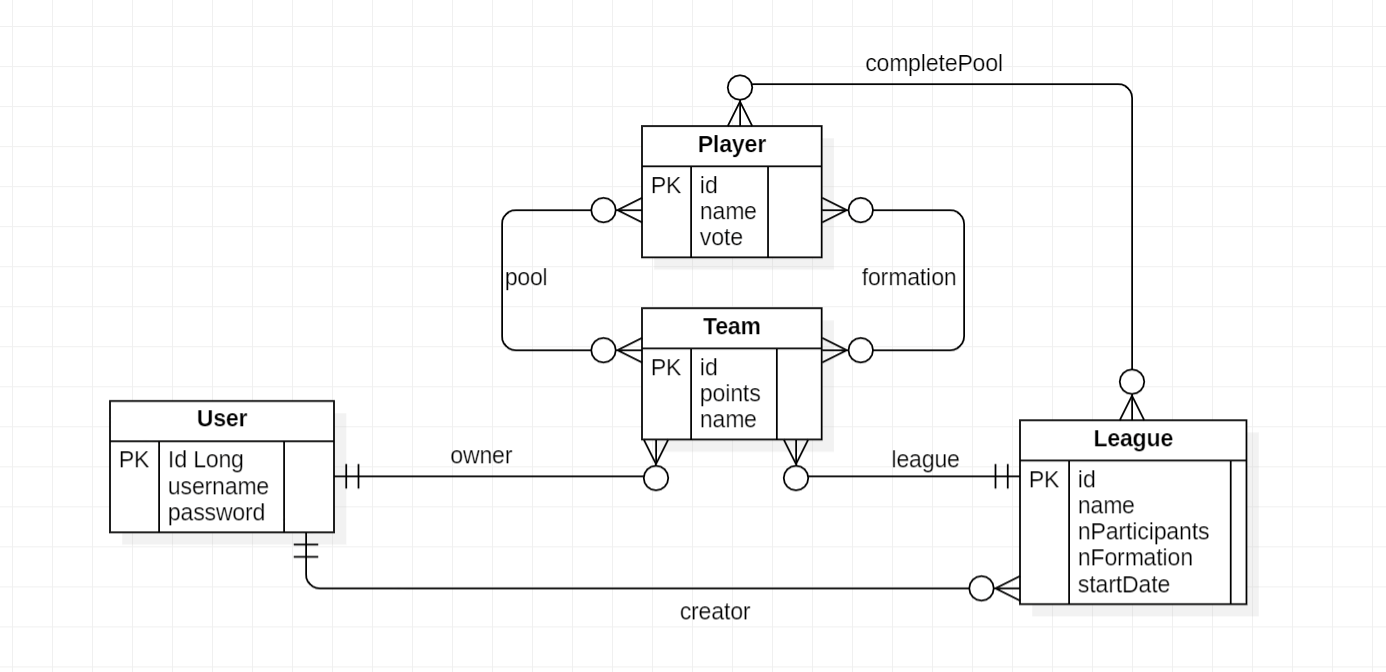
\includegraphics[width=\linewidth]{images/erDia.png}
  \caption{Entity Relationship Diagram}
  \label{fig:ER Diagram}
\end{figure}

\chapter{Implementazioni delle classi}
Abbiamo suddiviso il progetto in package Java: il modello dati nel package entities, la logica
di controllo nel package gui ed infine la gestione del Database nel package dao e repositories.
Il codice è suddiviso in tale modo:

\begin{figure}[H]
  \centering
  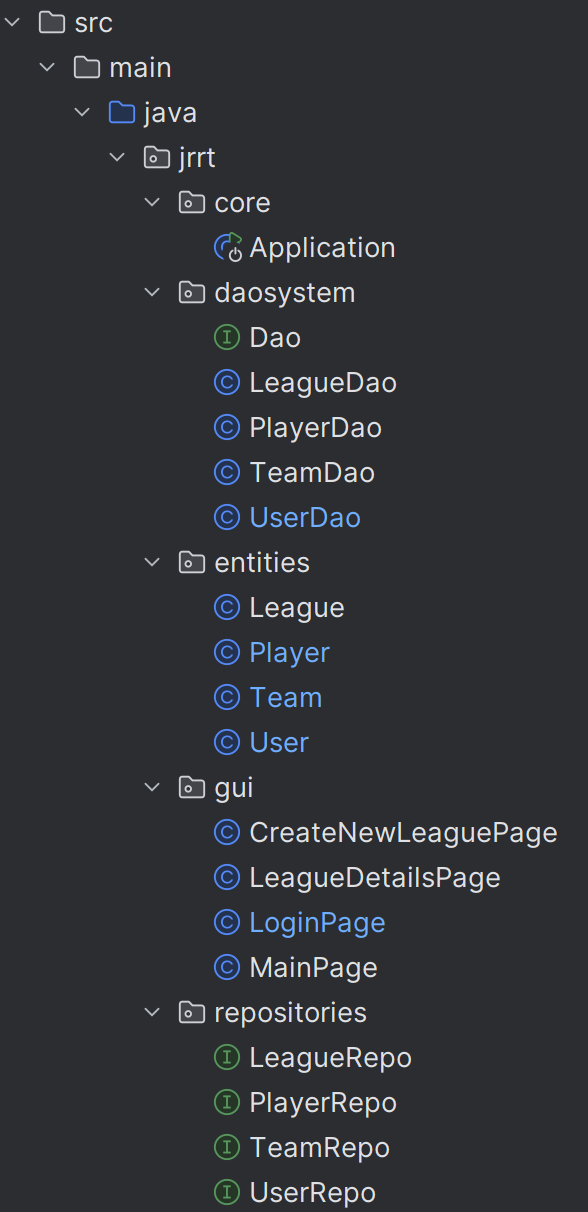
\includegraphics[width=60mm]{images/codeStruct.png}
  \caption{Suddivisione dei package}
  \label{fig:codeStructure}
\end{figure}

\section{entities}
Il package entities si occupa di definire un modello di composizione di classi su cui è possibile eseguire i casi d’uso espressi nello Use Case Diagram. Questo package si articola nelle
seguenti classi:

\subsection{User}
Lo User è un utente, che registrandosi alla webApp, può creare nuove leghe o partecipare ad altre create da altri User. Gli attributi sono:

\begin{itemize}
    \item id: un identificativo univoco dell'utente.
    \item username: una stringa che contiene il nickname con il quale l'utente vuole chiamarsi nel programma.
    \item password: una stringa relazionata allo username per permettere il login.
\end{itemize}

\subsection{Team} Il Team è una squadra, che viene creata quando un utente partecipa o crea una lega. Gli attributi sono:

\begin{itemize} 
    \item id: un identificativo univoco della squadra. 
    \item name: una stringa che contiene il nome della squadra. 
    \item points: un intero che rappresenta i punti accumulati dalla squadra durante tutto il campionato.
    \item owner: un oggetto User che rappresenta l'utente proprietario della squadra. 
    \item league: un oggetto League che rappresenta la lega a cui appartiene la squadra. 
    \item pool: un insieme di oggetti Player che rappresentano i giocatori disponibili per la squadra. 
    \item formation: un insieme di oggetti Player che rappresentano la formazione attuale della squadra per la prossima giornata.
\end{itemize}

\subsection{Player} 
Il Player è un giocatore, che può essere aggiunto a una squadra da il creatore della lega. Gli attributi sono:

\begin{itemize} 
    \item id: un identificativo univoco del giocatore. 
    \item name: una stringa che contiene il nome del giocatore. 
    \item vote: un intero che rappresenta il voto del giocatore nell'ultima partita. 
    \item leagues: un insieme di oggetti League che rappresentano le leghe a cui il giocatore appartiene. 
    \item teams: un insieme di oggetti Team che rappresentano le squadre a cui il giocatore appartiene come membro del pool. 
    \item teamsFormation: un insieme di oggetti Team che rappresentano le squadre in cui il giocatore è attualmente in formazione.
\end{itemize}

\subsection{League} 
La League è una lega, che può essere creata da un utente. Gli attributi sono:  

\begin{itemize} 
    \item id: un identificativo univoco della lega. 
    \item name: una stringa che contiene il nome della lega. 
    \item nParticipants: un intero che rappresenta il numero di partecipanti alla lega. 
    \item nFormation: un intero che rappresenta il numero di formazioni per squadra nella lega. 
    \item startDate: una data che rappresenta la data in cui viene calcolata la prossima giornata.
    \item creator: un oggetto User che rappresenta l'utente che ha creato la lega. 
    \item teams: un insieme di oggetti Team che rappresentano le squadre che partecipano alla lega. 
    \item completePool: un insieme di oggetti Player che rappresentano i giocatori disponibili per la lega. 
\end{itemize}

\section{gui}
Il package gui (Graphical User Interface) si occupa della gestione dell'interfaccia utente dell'applicazione. Questo package contiene le classi che definiscono come l'utente interagisce con l'applicazione, creando, modificando o elementi dell' entities, ma mai accedendo direttamente al DataBase.

\subsection{LoginPage}
La classe LoginPage è un controller Spring MVC che gestisce le operazioni di login e registrazione degli utenti. Ecco i principali metodi implementati nella classe: 

\begin{itemize}

    \item loginPage: Questo metodo gestisce le richieste GET alla radice dell'applicazione ("/"). Prepara un nuovo oggetto User e lo aggiunge al modello, quindi restituisce la vista "loginPage" per essere visualizzata. 
 
    \item signup: Questo metodo gestisce le richieste POST a "/signup". Prende un oggetto User come parametro, controlla se esiste già un utente con lo stesso nome utente nel database. Se non esiste, salva il nuovo utente nel database e restituisce la vista "loginPage" con un messaggio informativo. Se esiste, restituisce la vista "loginPage" con un messaggio di errore.  
    
    \item login: Questo metodo gestisce le richieste POST a "/login". Prende un oggetto User come parametro, cerca un utente con lo stesso nome utente nel database. Se l'utente esiste e la password corrisponde, imposta l'utente come l'utente attualmente loggato nella sessione e reindirizza alla pagina principale. Se l'utente non esiste o la password non corrisponde, restituisce la vista "loginPage" con un messaggio di errore. 

\end{itemize}

\subsection{MainPage} 
La classe MainPage è un controller Spring MVC che gestisce le operazioni principali dell'applicazione. Ecco i principali metodi implementati nella classe:  
\begin{itemize}  
    \item mainPage: Questo metodo gestisce le richieste GET a "/main". Rimuove l'attributo "league" dalla sessione, recupera l'utente attuale dalla sessione e, se l'utente non è null, recupera le leghe a cui l'utente partecipa, le ordina per data di inizio e le aggiunge al modello. Infine, restituisce la vista "mainPage" per essere visualizzata. 
    \item newLeague: Questo metodo gestisce le richieste GET a "/newLeague". Recupera l'utente e la lega dalla sessione. Se la lega è null, crea una nuova lega con valori predefiniti e la aggiunge alla sessione. Recupera i giocatori della lega e li aggiunge al modello. Infine, restituisce la vista "createNewLeaguePage" per essere visualizzata. 
    \item joinLeague: Questo metodo gestisce le richieste POST a "/joinLeague". Prende un parametro "leagueId" che rappresenta l'ID della lega a cui l'utente vuole unirsi. Recupera l'utente dalla sessione e la lega dal database. Se la lega esiste e non è piena, crea una nuova squadra con l'utente come proprietario e la lega come lega, salva la squadra nel database e reindirizza alla pagina principale. Se la lega non esiste o è piena, restituisce un messaggio di errore e reindirizza alla pagina principale.
\end{itemize}

\subsection{CreateNewLeaguePage} 
La classe CreateNewLeaguePage è un controller Spring MVC che gestisce la creazione di nuove leghe. Ecco i principali metodi implementati nella classe:  
\begin{itemize}
    \item createNewLeague: Questo metodo gestisce le richieste POST a "/createNewLeague". Prende un oggetto League come parametro, controlla se esiste già una lega con lo stesso nome nel database. Se non esiste, salva la nuova lega nel database, crea una nuova squadra con l'utente come proprietario e la lega come lega, salva la squadra nel database e rimuove l'attributo "league" dalla sessione. Infine, reindirizza alla pagina principale.
    \item addPlayerToLeaguePool: Questo metodo gestisce le richieste POST a "/addPlayer/{playerName}". Prende una stringa playerName come parametro, recupera l'utente e la lega dalla sessione. Se l'utente o la lega sono null, reindirizza alla pagina principale. Recupera il pool di giocatori della lega e controlla se esiste già un giocatore con lo stesso nome nel pool. Se esiste, restituisce un messaggio di errore e reindirizza alla pagina "newLeague". Se non esiste, crea un nuovo giocatore con il nome fornito, aggiunge il giocatore alla lega, salva il giocatore nel database e reindirizza alla pagina "newLeague".
\end{itemize}

\subsection{LeagueDetailsPage} 
La classe LeagueDetailsPage è una Spring MVC controller che funziona mostrando e gestendo tutti i dettagli specifici di una lega. Ecco i principali metodi implementati nella classe:  
\begin{itemize}  
    \item leagueDetails: Questo metodo gestisce le richieste GET a "/leagueDetails/{id}". Recupera l'utente e la lega dalla sessione. Se l'utente o la lega sono null, reindirizza alla pagina principale. Altrimenti, aggiunge l'utente, la lega, le squadre della lega e i giocatori della lega al modello. Infine, restituisce la vista "leagueDetailsPage" per essere visualizzata. 
    \item modifyLeague: Questo metodo gestisce le richieste GET a "/modifyLeague". Recupera l'utente e la lega dalla sessione. Se l'utente o la lega sono null, reindirizza alla pagina principale. Altrimenti, aggiunge l'utente, la lega, le squadre della lega e i giocatori della lega al modello. Infine, restituisce la vista "modifyLeaguePage" per essere visualizzata. 
    \item removeTeam: Questo metodo gestisce le richieste GET a "/removeTeam/{id}". Prende un parametro "id" che rappresenta l'ID della squadra da rimuovere. Recupera la squadra dal database e la rimuove. Se la lega non ha più squadre, rimuove anche la lega. Infine, reindirizza alla pagina "modifyLeague". 
    \item addPlayer: Questo metodo gestisce le richieste GET a "/addPlayer/{userId}/{teamId}". Prende due parametri "userId" e "teamId" che rappresentano l'ID dell'utente e l'ID della squadra rispettivamente. Recupera l'utente, la squadra e la lega dalla sessione. Se l'utente, la squadra o la lega sono null, reindirizza alla pagina principale. Altrimenti, aggiunge l'utente, la squadra e i giocatori della lega al modello. Infine, restituisce la vista "addPlayersPage" per essere visualizzata. 
    \item addPlayersToTeam: Questo metodo gestisce le richieste POST a "/addPlayersToTeam/{teamId}". Prende un parametro "teamId" che rappresenta l'ID della squadra e una lista di ID di giocatori. Aggiunge i giocatori alla squadra e salva la squadra nel database. Infine, reindirizza alla pagina "modifyLeague". 
    \item addPlayersToFormation: Questo metodo gestisce le richieste POST a "/addPlayersToFormation/{teamId}". Prende un parametro "teamId" che rappresenta l'ID della squadra e una lista di ID di giocatori. Aggiunge i giocatori alla formazione della squadra e salva la squadra nel database. Infine, reindirizza alla pagina "leagueDetails/{teamId}". 
    \item setVote: Questo metodo gestisce le richieste POST a "/setVote". Prende una serie di parametri che rappresentano i voti dei giocatori. Imposta il voto di ogni giocatore e salva il giocatore nel database. Infine, reindirizza alla pagina "modifyLeague". 
    \item evaluateDay: Questo metodo gestisce le richieste POST a "/EvaluateDay". Prende un parametro "newStartDate" che rappresenta la nuova data della prossima giornata. Aggiorna la data, calcola i punti di ogni squadra in base ai voti dei giocatori nelle varie formazioni e salva la lega nel database. Infine, reindirizza alla pagina "modifyLeague".
\end{itemize}

\section{daosystem}
Il package daosystem gestisce le connessioni e le operazioni sul database utilizzando il pattern DAO (Data Access Object). Questo pattern fornisce un'interfaccia astratta che consente di manipolare i dati dell'applicazione, indipendentemente dal sistema di persistenza dei dati sottostante. In questo caso, il sistema di persistenza dei dati è un database MySQL. MySQL è un sistema di gestione di database relazionale (RDBMS) open source che utilizza SQL (Structured Query Language) per l'accesso ai dati.  Il package daosystem utilizza anche il framework Spring Boot JPA (Java Persistence API) per semplificare l'accesso ai dati nel database. JPA è una specifica standard di Java che astrae i dettagli dell'accesso ai dati, permettendo agli sviluppatori di interagire con il database in modo più intuitivo e orientato agli oggetti.

\subsection{UserDao}
La classe UserDao si interfaccia con il database per la gestione della tabella degli utenti, separando l'oggetto User Java dall'entità corrispondente salvata nel database. Questa classe contiene la JPA Repository UserRepo e si occupa di inizializzarla. UserDao avvia il collegamento che mette in comunicazione il programma e il database, attraverso il passaggio del parametro ApplicationContext ottenuto una volta avviata l'applicazione. I principali metodi che vengono forniti da UserDao sono i seguenti:  \begin{itemize} 
    \item `save(User user)`: salva, attraverso la repository `UserRepo`, l'oggetto `User` nel database e notifica il successo dell'operazione. 
    \item `delete(User user)`: cancella, attraverso la repository `UserRepo`, l'oggetto `User` nel database e notifica il successo dell'operazione. 
    \item `getAll()`: fornisce un insieme contenente tutti gli oggetti `User` attualmente esistenti nel database. 
    \item `get(Long id)`: restituisce un'occorrenza di un oggetto `User` data la sua chiave primaria. 
    \item `getByName(String name)`: restituisce un'occorrenza di un oggetto `User` dato il suo nome. 
    \item `update(User user, String[] params)`: aggiorna, attraverso la repository `UserRepo`, l'oggetto `User` nel database e notifica il successo dell'operazione. </pre> 
\end{itemize}

\subsection{TeamDao} 
La classe TeamDao si interfaccia con il database per la gestione della tabella delle squadre, separando l'oggetto Team Java dall'entità corrispondente salvata nel database. Questa classe contiene la JPA Repository TeamRepo e si occupa di inizializzarla. TeamDao avvia il collegamento che mette in comunicazione il programma e il database, attraverso il passaggio del parametro ApplicationContext ottenuto una volta avviata l'applicazione. I principali metodi che vengono forniti da TeamDao sono i seguenti:  \begin{itemize}
    \item `save(Team team)`: salva, attraverso la repository `TeamRepo`, l'oggetto `Team` nel database e notifica il successo dell'operazione. 
    \item `delete(Team team)`: cancella, attraverso la repository `TeamRepo`, l'oggetto `Team` nel database e notifica il successo dell'operazione. 
    \item `getAll()`: fornisce un insieme contenente tutti gli oggetti `Team` attualmente esistenti nel database. 
    \item `get(Long id)`: restituisce un'occorrenza di un oggetto `Team` data la sua chiave primaria. 
    \item `getPlayers(Long Id)`: restituisce un insieme di oggetti `Player` che appartengono alla squadra con l'ID specificato. 
    \item `getByUserId(Long userId)`: restituisce un oggetto `Team` che appartiene all'utente con l'ID specificato. 
    \item `getTeamByOwnerAndLeague(User owner, League league)`: restituisce un oggetto `Team` che appartiene all'utente specificato e alla lega specificata. 
    \item `getPoolByTeamId(Long teamId)`: restituisce un insieme di oggetti `Player` che appartengono alla pool della squadra con l'ID specificato.  
\end{itemize}

\subsection{PlayerDao} 
La classe PlayerDao si interfaccia con il database per la gestione della tabella dei giocatori, separando l'oggetto Player Java dall'entità corrispondente salvata nel database. Questa classe contiene la JPA Repository PlayerRepo e si occupa di inizializzarla. PlayerDao avvia il collegamento che mette in comunicazione il programma e il database, attraverso il passaggio del parametro ApplicationContext ottenuto una volta avviata l'applicazione. I principali metodi che vengono forniti da PlayerDao sono i seguenti:  
\begin{itemize}  
    \item `save(Player player)`: salva, attraverso la repository `PlayerRepo`, l'oggetto `Player` nel database e notifica il successo dell'operazione. 
    \item `delete(Player player)`: cancella, attraverso la repository `PlayerRepo`, l'oggetto `Player` nel database e notifica il successo dell'operazione. 
    \item `getAll()`: fornisce un insieme contenente tutti gli oggetti `Player` attualmente esistenti nel database. 
    \item `get(Long id)`: restituisce un'occorrenza di un oggetto `Player` data la sua chiave primaria. 
    \item `getByName(String name)`: restituisce un'occorrenza di un oggetto `Player` dato il suo nome. 
    \item `getPlayersOfLeague(Long id)`: restituisce un insieme di oggetti `Player` che appartengono alla lega con l'ID specificato.  
\end{itemize}

\subsection{LeagueDao} 
La classe LeagueDao si interfaccia con il database per la gestione della tabella delle leghe, separando l'oggetto League Java dall'entità corrispondente salvata nel database. Questa classe contiene la JPA Repository LeagueRepo e si occupa di inizializzarla. LeagueDao avvia il collegamento che mette in comunicazione il programma e il database, attraverso il passaggio del parametro ApplicationContext ottenuto una volta avviata l'applicazione. I principali metodi che vengono forniti da LeagueDao sono i seguenti:  
\begin{itemize}  
    \item `save(League league)`: salva, attraverso la repository `LeagueRepo`, l'oggetto `League` nel database e notifica il successo dell'operazione. 
    \item `delete(League league)`: cancella, attraverso la repository `LeagueRepo`, l'oggetto `League` nel database e notifica il successo dell'operazione. 
    \item `getAll()`: fornisce un insieme contenente tutti gli oggetti `League` attualmente esistenti nel database. 
    \item `get(Long id)`: restituisce un'occorrenza di un oggetto `League` data la sua chiave primaria. 
    \item `getByName(String name)`: restituisce un insieme di oggetti `League` dato il loro nome. 
    \item `getPlayers(Long id)`: restituisce un insieme di oggetti `Player` che appartengono alla lega con l'ID specificato. 
    \item `getTeams(Long id)`: restituisce un insieme di oggetti `Team` che appartengono alla lega con l'ID specificato. 
    \item `getUserAttendedLeagues(Long id)`: restituisce un insieme di oggetti `League` a cui l'utente con l'ID specificato ha partecipato.
\end{itemize}

\section{repositories}
Il package repositories è un componente fondamentale nell'architettura di un'applicazione Spring Boot. Questo package contiene le interfacce che estendono CrudRepository o JpaRepository, che forniscono metodi CRUD (Create, Read, Update, Delete) per l'accesso ai dati.  Ogni interfaccia nel package repositories corrisponde a un'entità nel database. Ad esempio, UserRepo corrisponde all'entità User, LeagueRepo corrisponde all'entità League, e così via. Queste interfacce definiscono metodi per eseguire operazioni sul database relative alle loro entità corrispondenti.  Questi metodi includono operazioni standard come save, delete, findAll, e findById. Inoltre, è possibile definire metodi personalizzati per eseguire query specifiche sul database. Ad esempio, UserRepo ha un metodo getByName che restituisce un User in base al suo nome.  Spring Data JPA implementa automaticamente queste interfacce quando l'applicazione viene eseguita. Ciò significa che non è necessario scrivere l'implementazione di questi metodi; Spring Data JPA genera l'implementazione basandosi sul nome del metodo.

\section{resurces}
Il folder resources è una directory speciale in un progetto Spring Boot che viene utilizzata per contenere file non-Java, come configurazioni, file di proprietà, file HTML, CSS, JavaScript, e immagini. Questi file sono utilizzati per vari scopi come la configurazione dell'applicazione, l'interfaccia utente, ecc.  
\subsection{static}
Il package static è una directory speciale all'interno di resources che viene utilizzata per servire contenuti statici come CSS, JavaScript, immagini e altri file multimediali. Spring Boot configura automaticamente Spring MVC per servire i file statici da questa directory. Ad esempio, il file style.css all'interno del package static/css contiene le definizioni di stile CSS utilizzate per formattare l'interfaccia utente dell'applicazione.  
\subsection{templates}
Il package templates è un'altra directory speciale all'interno di resources che viene utilizzata per contenere i file di template. Questi file di template sono utilizzati per generare dinamicamente il codice HTML che viene inviato al browser. Spring Boot utilizza un motore di templating, come Thymeleaf o FreeMarker, per processare questi file di template. Ad esempio, i file .html all'interno del package templates contengono il codice HTML che definisce la struttura delle pagine web dell'applicazione.

\chapter{Test (JUnit) }
JUnit è un framework di testing per il linguaggio di programmazione Java. È utilizzato per scrivere e eseguire test automatizzati per verificare che il codice si comporti come previsto. Ogni test è indipendente dagli altri. Prima di ogni test, il database è ripulito e preparato per il test successivo. Questo garantisce che i test non influenzino l'uno l'altro e che ogni test sia ripetibile.

\section{UserTest}
Nel contesto del UserTest fornito, JUnit viene utilizzato per testare il comportamento della classe UserDao. Ogni metodo annotato con @Test è un caso di test indipendente.  Ecco una breve descrizione di come funzionano i test in UserTest: 

\begin{itemize}   
    \item contextLoads(): Questo test verifica che l'istanza di UserDao sia stata correttamente iniettata nel test. Se UserDao è null, il test fallisce.  
    testNumberOfUsers(): Questo test verifica che il metodo getAll() di UserDao restituisca il numero corretto di utenti. Crea un certo numero di utenti, li salva nel database, quindi verifica che il numero di utenti restituiti da getAll() sia uguale al numero di utenti creati.  
    \item testUserCreation(): Questo test verifica che un utente possa essere correttamente salvato nel database. Crea un nuovo utente, lo salva nel database, quindi cerca l'utente nel database per nome e verifica che i dettagli dell'utente corrispondano.  
    testUserDeletion(): Questo test verifica che un utente possa essere correttamente eliminato dal database. Crea un nuovo utente, lo salva nel database, lo elimina, quindi cerca l'utente nel database per nome e verifica che l'utente non esista più.  
    \item testModifyUser(): Questo test verifica che i dettagli di un utente possano essere correttamente modificati. Crea un nuovo utente, lo salva nel database, modifica i dettagli dell'utente, lo salva di nuovo, quindi cerca l'utente nel database per nome e verifica che i dettagli dell'utente siano stati aggiornati. 
\end{itemize}

\begin{figure}[H]
  \centering
  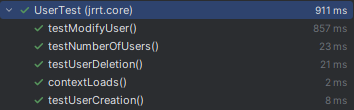
\includegraphics[width=60mm]{images/userTest.png}
  \caption{User test eseguiti con esito positivo}
  \label{fig:userTests}
\end{figure}

\section{TeamTest} 
Nel contesto del TeamTest fornito, JUnit viene utilizzato per testare il comportamento della classe TeamDao. Ogni metodo annotato con @Test è un caso di test indipendente. Ecco una breve descrizione di come funzionano i test in TeamTest:  
\begin{itemize}
    \item contextLoads(): Questo test verifica che l'istanza di TeamDao, UserDao, LeagueDao e PlayerDao siano state correttamente iniettate nel test. Se una di queste è null, il test fallisce. \item testTeamCreation(): Questo test verifica che un team possa essere correttamente salvato nel database. Crea un nuovo utente, una nuova lega e un nuovo team, li salva nel database, quindi cerca il team nel database per ID e verifica che i dettagli del team corrispondano. 
    \item testTeamDeletion(): Questo test verifica che un team possa essere correttamente eliminato dal database. Crea un nuovo utente, una nuova lega e un nuovo team, li salva nel database, elimina il team, quindi cerca il team nel database per ID e verifica che il team non esista più. 
    \item testModifyTeam(): Questo test verifica che i dettagli di un team possano essere correttamente modificati. Crea un nuovo utente, una nuova lega e un nuovo team, li salva nel database, modifica i dettagli del team, lo salva di nuovo, quindi cerca il team nel database per ID e verifica che i dettagli del team siano stati aggiornati. 
    \item testGetTeamByOwnerAndLeague(): Questo test verifica che il metodo getTeamByOwnerAndLeague di TeamDao restituisca il team corretto. Crea un nuovo utente, una nuova lega e un nuovo team, li salva nel database, quindi chiama il metodo getTeamByOwnerAndLeague e verifica che il team restituito corrisponda al team creato. 
    \item testGetPoolByTeamId(): Questo test verifica che il metodo getPoolByTeamId di TeamDao restituisca l'insieme corretto di giocatori. Crea un nuovo utente, una nuova lega, un nuovo team e due nuovi giocatori, li salva nel database, aggiunge i giocatori al team, quindi chiama il metodo getPoolByTeamId e verifica che l'insieme di giocatori restituito corrisponda ai giocatori aggiunti al team. 
\end{itemize}  
\begin{figure}[H] 
\centering 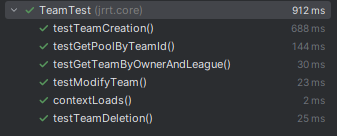
\includegraphics[width=60mm]{images/teamTest.png} \caption{Team test eseguiti con esito positivo} \label{fig:teamTests} \end{figure}

\section{PlayerTest} 
Nel contesto del PlayerTest fornito, JUnit viene utilizzato per testare il comportamento della classe PlayerDao. Ogni metodo annotato con @Test è un caso di test indipendente. Ecco una breve descrizione di come funzionano i test in PlayerTest:  \begin{itemize} 
    \item contextLoads(): Questo test verifica che l'istanza di PlayerDao sia stata correttamente iniettata nel test. Se PlayerDao è null, il test fallisce. 
    \item testPlayerCreation(): Questo test verifica che un giocatore possa essere correttamente salvato nel database. Crea un nuovo giocatore, lo salva nel database, quindi cerca il giocatore nel database per ID e verifica che i dettagli del giocatore corrispondano. 
    \item testPlayerDeletion(): Questo test verifica che un giocatore possa essere correttamente eliminato dal database. Crea un nuovo giocatore, lo salva nel database, lo elimina, quindi cerca il giocatore nel database per ID e verifica che il giocatore non esista più. 
    \item testModifyPlayer(): Questo test verifica che i dettagli di un giocatore possano essere correttamente modificati. Crea un nuovo giocatore, lo salva nel database, modifica i dettagli del giocatore, lo salva di nuovo, quindi cerca il giocatore nel database per ID e verifica che i dettagli del giocatore siano stati aggiornati. 
\end{itemize}  
\begin{figure}[H] 
\centering 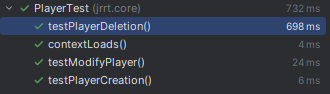
\includegraphics[width=60mm]{images/playerTest.png} \caption{Player test eseguiti con esito positivo} \label{fig:playerTests} 
\end{figure}

\section{LeagueTest} 
Nel contesto del LeagueTest fornito, JUnit viene utilizzato per testare il comportamento della classe LeagueDao. Ogni metodo annotato con @Test è un caso di test indipendente. Ecco una breve descrizione di come funzionano i test in LeagueTest:  \begin{itemize} 
    \item contextLoads(): Questo test verifica che l'istanza di LeagueDao, UserDao e PlayerDao siano state correttamente iniettate nel test. Se una di queste è null, il test fallisce. 
    \item testLeagueCreation(): Questo test verifica che una lega possa essere correttamente salvata nel database. Crea un nuovo utente e una nuova lega, li salva nel database, quindi cerca la lega nel database per ID e verifica che i dettagli della lega corrispondano. 
    \item testLeagueDeletion(): Questo test verifica che una lega possa essere correttamente eliminata dal database. Crea un nuovo utente e una nuova lega, li salva nel database, elimina la lega, quindi cerca la lega nel database per ID e verifica che la lega non esista più. 
    \item testGetUserAttendedLeagues(): Questo test verifica che il metodo getUserAttendedLeagues di LeagueDao restituisca le leghe corrette. Crea un nuovo utente e due nuove leghe, li salva nel database, quindi chiama il metodo getUserAttendedLeagues e verifica che le leghe restituite corrispondano alle leghe create. \end{itemize}  
\begin{figure}[H] 
\centering 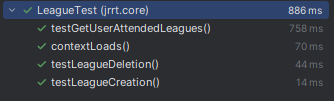
\includegraphics[width=60mm]{images/leagueTest.png} \caption{League test eseguiti con esito positivo} \label{fig:leagueTests} 
\end{figure}



















\end{document}

